\documentclass[output=paper,colorlinks,citecolor=brown
% ,hidelinks
% showindex
]{langscibook}
\author{Delia Bentley\orcid{}\affiliation{University of Manchester}}
\title[The causative alternation in Italian]{The causative alternation in Italian: A case study in the parallel architecture of grammar}
\abstract{In this article we discuss corpus evidence from Italian which suggests that the causative alternation cannot be reduced to a single principle, be it semantic, syntactic or at the interface between these two levels of analysis. We argue that the boundaries of the causative alternation are established in grammar through (i) the acquisition of inchoative and causative logical structures, which are stored in the lexicon alongside non-templatic facets of meaning, (ii) general semantics-syntax mapping principles, which are subject to 
alignment variation, and (iii) constructional instructions, which determine which subclasses of verbs can enter the constructions that are relevant to the causative alternation in each individual language. Two such constructions are identified in our study of Italian, the one being marked by the morpheme \textsc{\textsc{se}}, the other being labile, though we suggest that the \textsc{-\textsc{se}} intransitives of alternating verbs are not necessarily anticausative. Our study reveals the causative alternation to be a prime illustration of the parallel architecture of grammar, where the default principles that govern the interplay of a rich lexical module with syntax interact with language specific constructional requirements.}


\IfFileExists{../localcommands.tex}{
   \addbibresource{../localbibliography.bib}
   \newcommand{\orcid}[1]{}

\usepackage{orcidlink}

\usepackage{tabularx,multicol}
\usepackage{url}
\urlstyle{same}


\usepackage{langsci-optional}
\usepackage{langsci-lgr}
\usepackage{langsci-gb4e}

% for texlive 2022
\usepackage{langsci-branding} 

% Müller


% \usepackage{biblatex-series-number-checks}

% \usepackage{eng-date}

% \usepackage{german}%% Das Buch ist nicht deutsch. Hör auf, solche Sachen zu laden


% \usepackage{tikz-dependency}
% \usepackage{tikz}
% \usepackage{tikz-qtree}

% \usepackage{hologo}

% 3_pullum.tex

% This does not work complains about recommanding epsilon
% We use a special adapted version, which is in the repro.
\usepackage{langsci-textipa}



% 8_levine

\usepackage{./styles/lg-macro2}
\usepackage{bm}
\usepackage{umoline}
\usepackage{pifont}
\usepackage{pstricks,pst-node,pst-tree}
\usepackage{ulem}
\usepackage{mathrsfs}
\usepackage{bussproofs}




%\usepackage{tikz,tikz-qtree}

%\usepackage{gb4e0}
%\noautomath

%\usepackage[letterpaper,margin=1.2in]{geometry}



% 14_kornai

%\usepackage{xypic} % seems not to be needed
% \usepackage[matrix,arrow]{xy}
%\usepackage{amsmath}
% \usepackage{subcaption}
% \usepackage{wrapfig}


   
\SetupAffiliations{output in groups = false,
                   orcid placement = after,
                   separator between two = {\bigskip\\},
                   separator between multiple = {\bigskip\\},
                   separator between final two = {\bigskip\\}
                   }

% ORCIDs in langsci-affiliations 
\definecolor{orcidlogocol}{cmyk}{0,0,0,1}
\RenewDocumentCommand{\LinkToORCIDinAffiliations}{ +m }
  {%
    \,\orcidlink{#1}%
  }


\makeatletter
\let\thetitle\@title
\let\theauthor\@author
\makeatother

\newcommand{\togglepaper}[1][0]{
   \bibliography{../localbibliography}
   \papernote{\scriptsize\normalfont
     \theauthor.
     \titleTemp.
     To appear in:
     E. Di Tor \& Herr Rausgeberin (ed.).
     Booktitle in localcommands.tex.
     Berlin: Language Science Press. [preliminary page numbering]
   }
   \pagenumbering{roman}
   \setcounter{chapter}{#1}
   \addtocounter{chapter}{-1}
}

\newbool{bookcompile}
\booltrue{bookcompile}
\newcommand{\bookorchapter}[2]{\ifbool{bookcompile}{#1}{#2}}


% Cite and cross-reference other chapters
\newcommand{\crossrefchaptert}[2][]{\citet*[#1]{chapters/#2}, Chapter~\ref{chap-#2} of this volume} 
\newcommand{\crossrefchapterp}[2][]{(\citealp*[#1]{chapters/#2}, Chapter~\ref{chap-#2} of this volume)}
\newcommand{\crossrefchapteralt}[2][]{\citealt*[#1]{chapters/#2}, Chapter~\ref{chap-#2} of this volume}
\newcommand{\crossrefchapteralp}[2][]{\citealp*[#1]{chapters/#2}, Chapter~\ref{chap-#2} of this volume}

\newcommand{\crossrefcitet}[2][]{\citet*[#1]{chapters/#2}} 
\newcommand{\crossrefcitep}[2][]{\citep*[#1]{chapters/#2}}
\newcommand{\crossrefcitealt}[2][]{\citealt*[#1]{chapters/#2}}
\newcommand{\crossrefcitealp}[2][]{\citealp*[#1]{chapters/#2}}


\newcommand{\sub}[1]{\textsubscript{\scriptsize\textrm{#1}}}

% Müller

\newcommand{\page}{}

\let\citew\citet

\def\underRevision{Revise and resubmit}

\let\textbfemph\emph

\newcommand{\todostefan}[1]{\todo[color=orange!80]{\footnotesize #1}\xspace}
\newcommand{\todosatz}[1]{\todo[color=red!40]{\footnotesize #1}\xspace}

\newcommand{\inlinetodostefan}[1]{\todo[color=green!40,inline]{\footnotesize #1}\xspace}

\newcommand{\inlinetodoopt}[1]{\todo[color=green!40,inline]{\footnotesize #1}\xspace}
\newcommand{\inlinetodoobl}[1]{\todo[color=red!40,inline]{\footnotesize #1}\xspace}

\newcommand{\itd}[1]{\inlinetodoobl{#1}}
\newcommand{\itdobl}[1]{\inlinetodoobl{#1}}
\newcommand{\itdopt}[1]{\inlinetodoopt{#1}}

\newcommand{\addpages}{\todostefan{add pages}}

%% % taken from https://tex.stackexchange.com/a/95079/18561
\newbox\usefulbox

\makeatletter
\def\getslant #1{\strip@pt\fontdimen1 #1}

\def\skoverline #1{\mathchoice
 {{\setbox\usefulbox=\hbox{$\m@th\displaystyle #1$}%
    \dimen@ \getslant\the\textfont\symletters \ht\usefulbox
    \divide\dimen@ \tw@ 
    \kern\dimen@ 
    \overline{\kern-\dimen@ \box\usefulbox\kern\dimen@ }\kern-\dimen@ }}
 {{\setbox\usefulbox=\hbox{$\m@th\textstyle #1$}%
    \dimen@ \getslant\the\textfont\symletters \ht\usefulbox
    \divide\dimen@ \tw@ 
    \kern\dimen@ 
    \overline{\kern-\dimen@ \box\usefulbox\kern\dimen@ }\kern-\dimen@ }}
 {{\setbox\usefulbox=\hbox{$\m@th\scriptstyle #1$}%
    \dimen@ \getslant\the\scriptfont\symletters \ht\usefulbox
    \divide\dimen@ \tw@ 
    \kern\dimen@ 
    \overline{\kern-\dimen@ \box\usefulbox\kern\dimen@ }\kern-\dimen@ }}
 {{\setbox\usefulbox=\hbox{$\m@th\scriptscriptstyle #1$}%
    \dimen@ \getslant\the\scriptscriptfont\symletters \ht\usefulbox
    \divide\dimen@ \tw@ 
    \kern\dimen@ 
    \overline{\kern-\dimen@ \box\usefulbox\kern\dimen@ }\kern-\dimen@ }}%
 {}}
\makeatother

% 1_intro.tex

% For the block quote:

\usepackage[most]{tcolorbox}
\definecolor{linequote}{RGB}{224,215,188}
\definecolor{backquote}{RGB}{249,245,233}
\newtcolorbox{myquote}[1][]{%
    enhanced, breakable, 
    size=minimal,
    frame hidden, boxrule=0pt,
    sharp corners,
    colback=backquote,
    #1
}

% 2_gibson.tex


% Example(s) Environments
% 12pt, No new-lines after example number is printed

\newcounter{examplectr}
\newcounter{fnexamplectr}

% Note: don't use subexamples in footnotes.

% This line is to overcome a bug in cmu-art style: it prints counter
% values to the aux file using \theaux... rather than using \the...
\def\theauxexamplectr{\theexamplectr}

\newcounter{subexamplectr}
\def\theauxsubexamplectr{\thesubexamplectr}
\def\theauxfnexamplectr{\thefnexamplectr}

\renewcommand{\theexamplectr}{\arabic{examplectr}}
% This command causes example numbers to appear without following periods

\renewcommand{\thefnexamplectr}{\roman{fnexamplectr}}
% This command causes example numbers to appear without following periods

\renewcommand{\thesubexamplectr}{\theexamplectr\alph{subexamplectr}}
% This command gives the number of an example and subexample as e.g. 1a, 2b

\newlength{\wdth}
\newcommand{\strike}[1]{\settowidth{\wdth}{#1}\rlap{\rule[.5ex]{\wdth}{1pt}}#1}

\newcommand{\exref}[1]{(\ref{#1})}
% This command puts reference numbers with parentheses
% surrounding them 

% The environment ``examples'' gives a list of examples, one on each line,
% numbered with a lower case alphabetic character
\newenvironment{examples}%
   { \vspace{-\baselineskip}
     \begin{list}%
     \textrm{\alph{subexamplectr}.}%
     {\usecounter{subexamplectr}
     \setlength{\topsep}{-\parskip}
     \setlength{\itemsep}{-2pt}
     \setlength{\leftmargin}{0.5in}
     \setlength{\rightmargin}{0in} } }%
   { \end{list}}

% The environment ``myexample'' outputs an arabic counter ``examplectr''
% surrounded by parentheses.
\newenvironment{myexample}
   { \vspace{20pt}
     \noindent
     \begin{minipage}{\textwidth}    % minipage environment disallows
                 % breaks across pages

     \refstepcounter{examplectr}     % step the counter and cause this
                 % section to be referenced by the
                 % counter ``examplectr''
     (\arabic{examplectr})}%
   { \vspace{20pt}
     \end{minipage}}

\newenvironment{myfnexample}
   { \vspace{2pt}
     \noindent
     \begin{minipage}{\textwidth}    % minipage environment disallows
                 % breaks across pages

     \refstepcounter{fnexamplectr}     % step the counter and cause this
                 % section to be referenced by the
                 % counter ``examplectr''
     (\roman{fnexamplectr})}%
   { \vspace{2pt}c
     \end{minipage}}
    
\newcommand*\circled[1]{\tikz[baseline=(char.base)]{
            \node[shape=circle,draw,inner sep=2pt] (char) {#1};}}



% 3_pullum.tex


% %%%  GKP:  I put in these pointless commands to kill off a bug elsewhere
% %%%        that tries to \newcommand \it (etc.) as \itshape (etc.), but
% %%%        fails because they haven't been defined.
% \newcommand{\it}{\relax}
% \newcommand{\bf}{\relax}
% \newcommand{\sc}{\relax}
% \newcommand{\rm}{\relax}

%%% GKP:  Two additional commands that I need
\newcommand{\data}[1]{\textit{#1}}
\newcommand{\blank}{\rule{1.2em}{0.5pt}}



% 8_levine

% ???
%\renewcommand{\emph}{\textit}
%\renewcommand{\em}{\it}

% not used \newcommand{\cites}[1]{\citeauthor{#1}'s~\citeyearpar{#1}}

% \renewcommand{\SetInfLen}{\setpremisesend{0pt}\setpremisesspace{10pt}\setnamespace{0pt}}

\newcommand{\pt}[1]{\ensuremath{\mathsf{#1}}}
\newcommand{\ptv}[1]{\ensuremath{\textsf{\textsl{#1}}}}

%\newcommand{\sv}[1]{\ensuremath{\bm{\mathcal{#1}}}}
\newcommand{\sv}[1]{\ensuremath{\mathcal{#1}}}

\newcommand{\sX}{\sv{X}}
\newcommand{\sF}{\sv{F}}
\newcommand{\sG}{\sv{G}}
%
% \renewcommand{\lex}{\SF}
% \renewcommand{\syncat}[1]{\ensuremath{\mathrm{#1}}}
% \newcommand{\syncatVar}[1]{\ensuremath{\mathit{#1}}}
%
% \newcommand{\RuleName}[1]{\textrm{#1}}
%
% \newcommand{\SemTyp}{\textsf{Sem}}
%
% \newcommand{\something}{\vdots\,\,\,\,\,\,\vdots}
%
% \newcommand{\pb}{\phantom{[}}
%
% \renewcommand{\E}{\ensuremath{\bm{\epsilon}}\xspace}
%
% \newcommand{\greeka}{\upalpha}
% \newcommand{\greekb}{\upbeta}
% \newcommand{\greekd}{\updelta}
\newcommand{\greekp}{\upvarphi}
\newcommand{\greekr}{\uprho}
\newcommand{\greeks}{\upsigma}
% \newcommand{\greekt}{\uptau}
% \newcommand{\greeko}{\upomega}
% \newcommand{\greekz}{\upzeta}
%
% % Do not do this!!!!!
% % \renewcommand{\labelenumi}{(\roman{enumi})}
%
% \newcommand{\upa}[2]{\ensuremath{\syncat{#1}|\syncat{#2}}}
% \newcommand{\dna}[2]{\upa{#2}{#1}}
%

%
% \newcommand{\Lemma}{\ensuremath{\vdots\hskip.5cm\vdots}\noLine}
%
% \newcommand{\la}{\ensuremath{\langle}}
% \newcommand{\ra}{\ensuremath{\rangle}}
%
% \renewcommand{\I}{\iota}
%
% \renewcommand{\sem}{\ensuremath}
%
% \newcommand{\LemmaShort}{\ensuremath{\vdots\hskip.2cm\vdots\hskip.2cm\vdots}\noLine}
% \newcommand{\LemmaShortAlt}{\ensuremath{\vdots\hskip.2cm\vdots}}
%
%
% \newcommand{\NoSem}{%
% \renewcommand{\LexEnt}[3]{##1; \syncat{##3}}
% \renewcommand{\LexEntTwoLine}[3]{\renewcommand{\arraystretch}{.8}%
% \begin{array}[b]{l} ##1;  \\ \syncat{##3} \end{array}}
% \renewcommand{\LexEntThreeLine}[3]{\renewcommand{\arraystretch}{.8}%
% \begin{array}[b]{l} ##1; \\ \syncat{##3} \end{array}}}
%
%
% \newcommand{\NoSemVar}{%
% \renewcommand{\LexEnt}[3]{##1; \syncat{##3}}
% \renewcommand{\LexEntTwoLine}[3]{\renewcommand{\arraystretch}{.8}%
% \begin{array}{l} ##1;  \\ \syncat{##3} \end{array}}
% \renewcommand{\LexEntThreeLine}[3]{\renewcommand{\arraystretch}{.8}%
% \begin{array}{l} ##1; \\ \syncat{##3} \end{array}}}
%
% \newcommand{\vs}{\raisebox{.05em}{\ensuremath{\upharpoonright}}}
%
% \newcommand{\AXX}[1]{\raisebox{-7mm}{\ensuremath{#1}}}
%
% \newcommand{\hypml}[2]{\left[\!\!#1\!\!\right]^{#2}}
%
% \newcommand{\alt}[2]{$\left\{\begin{array}{c}
% \hskip-.7ex\textrm{#1}\hskip-.7ex \\
% \hskip-.7ex\textrm{#2}\hskip-.7ex
%         \end{array}
% \right\}$}
%
% \newcommand{\altalt}[2]{\{#1/#2\}}
%
%
%
% \newcommand{\altt}[3]{$\left\{\begin{array}{c}
% \hskip-.7ex\textrm{#1}\hskip-.7ex \\
% \hskip-.7ex\textrm{#2}\hskip-.7ex \\
% \hskip-.7ex\textrm{#3}\hskip-.7ex
% \end{array}
% \right\}$}
%
% \newcommand{\alttt}[4]{$\left\{\begin{array}{c}
% \hskip-.7ex\textrm{#1}\hskip-.7ex \\
% \hskip-.7ex\textrm{#2}\hskip-.7ex \\
% \hskip-.7ex\textrm{#3}\hskip-.7ex \\
% \hskip-.7ex\textrm{#4}\hskip-.7ex
% \end{array}
% \right\}$}
%
%
% %%%%for bussproof
%
% \def\defaultHypSeparation{\hskip0.1in}
% \def\ScoreOverhang{0pt}
%
%
% %%\newcommand{\MultiLine}[1]{\renewcommand{\arraystretch}{.8}%
% %%\ensuremath{\begin{array}{l} #1 \end{array}}}
%
\newcommand{\MultiLine}[1]{\renewcommand{\arraystretch}{.8}%
\ensuremath{\begin{array}[b]{l} #1 \end{array}}}

%
%
% \newcommand{\MultiLineMod}[1]{%
% \ensuremath{\begin{array}[t]{l} #1 \end{array}}}
%
%
% %%%%%\AFourMargin
% %%\JLSubmissionMargin
%
% %%\setlength\topmargin{-1cm}
% %%\setlength\textheight{23cm}
% %%%%%\setlength\textwidth{13.5cm}
%
% %\setstretch{1.2}
%
% % not used \newcommand{\hyp}[2]{[ #]^{#2}}
%
\newcommand{\LexEnt}[3]{#1; \ensuremath{#2}; \syncat{#3}}
%
% \newcommand{\LexEntTwoLine}[3]{\renewcommand{\arraystretch}{.8}%
% \begin{array}[b]{l} #1; \\ \ensuremath{#2};  \syncat{#3} \end{array}}
%
% \newcommand{\LexEntThreeLine}[3]{\renewcommand{\arraystretch}{.8}%
% \begin{array}[b]{l} #1; \\ \ensuremath{#2}; \\ \syncat{#3} \end{array}}
%
%
% \newcommand{\LexEntFiveLine}[5]{\renewcommand{\arraystretch}{.8}%
% \begin{array}{l} #1 \\ #2; \\ \ensuremath{#3} \\ \ensuremath{#4}; \\ \syncat{#5} \end{array}}
%
%
% \newcommand{\LexEntFourLine}[4]{\renewcommand{\arraystretch}{.8}%
% \begin{array}{l} \pt{#1} \\ \pt{#2}; \\ \syncat{#4} \end{array}}
%
% \newcommand{\ManySomething}{\renewcommand{\arraystretch}{.8}%
% \raisebox{-3mm}{\begin{array}[b]{c} \vdots \,\,\,\,\,\, \vdots \\
% \vdots \,\,\,\,\,\, \vdots \end{array}}}
%
%
% \newcommand{\lemma}[1]{\renewcommand{\arraystretch}{.8}%
% \begin{array}[b]{c} \vdots \,\,\,\,\,\, \vdots \\ #1 \end{array}}
%
% \newcommand{\lemmarev}[1]{\renewcommand{\arraystretch}{.8}%
% \begin{array}[b]{c} #1 \\ \vdots \,\,\,\,\,\, \vdots \end{array}}
%
% \newcommand{\p}{\ensuremath{\upvarphi}}
%
% \newcommand{\Not}{\leavevmode\llap{\textbf{\smc{NOT:}} }}
%
% \newcommand{\Conj}{\fs{\bsp{\mathit{X}}{\mathit{X}}}{\mathit{X}}}
% \newcommand{\ConjY}{\fs{\bsp{\mathit{Y}}{\mathit{Y}}}{\mathit{Y}}}
% \newcommand{\sameLE}{\dna{(\upa{(\upa{S}{\mathit{X}})}{NP})}{(\upa{S}{\mathit{X}})}}
%
% \newcommand{\derivcenter}[2][1.1]{%
% \SetInfLen
% \attop{\vskip3ex
% \resizebox{#1\linewidth}{!}{\hskip-#1in
% #2}}}
%
% \newcommand{\derivcenterAlt}[2][.98]{%
% \SetInfLen
% \attop{\vskip3ex
% \resizebox{#1\linewidth}{!}{\hskip-#1in \hskip.5in
% #2}}\vspace{.5ex}}
%
% \renewcommand{\O}{\circ}  Do not recommand!
\newcommand{\BobsO}{\circ}
%
% \newcommand{\derivcenterMod}[2][1.1]{%
% \renewcommand{\LexEntThreeLine}[3]{\renewcommand{\arraystretch}{.8}%
% \raisebox{.4ex}{\ensuremath{\begin{array}{l} ##1; \\ \ensuremath{##2}; \\ \syncat{##3} \end{array}}}}
% \SetInfLen
% \attop{\vskip3ex
% \resizebox{#1\linewidth}{!}{\hskip-#1in
% #2}}}
%
%
% \newcommand{\shortarrow}{\xspace\hskip-1.2ex\scalebox{.5}[1]{\ensuremath{\bm{\rightarrow}}}\hskip-.5ex\xspace}
%
% \newcommand{\SemInt}[1]{\mbox{$[\![ \textrm{#1} ]\!]$}}
%
% \def\maru#1{{\ooalign{\hfil
%   \ifnum#1>999 \resizebox{.25\width}{\height}{#1}\else%
%   \ifnum#1>99 \resizebox{.33\width}{\height}{#1}\else%
%   \ifnum#1>9 \resizebox{.5\width}{\height}{#1}\else #1%
%   \fi\fi\fi%
% \/\hfil\crcr%
% \raise.167ex\hbox{\mathhexbox20D}}}}
%
\newcommand{\HypSpace}{\hskip-.8ex}
\newcommand{\RaiseHeight}{\raisebox{2.2ex}}
% \newcommand{\RaiseHeightLess}{\raisebox{1ex}}
%
% \newcommand{\fW}{\ensuremath{\mathfrak{W}}}
%
\newcommand{\ThreeColHyp}[1]{\RaiseHeight{\Bigg[}\HypSpace#1\HypSpace\RaiseHeight{\Bigg]}}
% \newcommand{\TwoColHyp}[1]{\RaiseHeightLess{\Big[}\HypSpace#1\HypSpace\RaiseHeightLess{\Big]}}
%
%
% %\newcommand{\maskref}[1]{\textsl{\textbf{[reference omitted for refereeing]}}}
% \newcommand{\maskref}[1]{#1}
%
% \newcommand{\DerivSize}{\small}
% \newcommand{\AppDerivSize}{\footnotesize}
%
% \renewcommand{\sem}{\ensuremath}


% \newcommand{\greekp}{{\color{green}π}}
% \newcommand{\greekr}{{\color{green}\textrho}}
% \newcommand{\greeks}{{\color{green}\textsigma}}
\newcommand{\ptfont}[1]{\texttt{#1}}                % what does ptfont do? Where is it defined?
                                % Question
%\newcommand{\ptfont}{\ttfamily}

%\newcommand{\grey}{\color{gray}}
\newcommand{\grey}[1]{\colorbox{mycolor}{#1}}
\definecolor{mycolor}{gray}{0.8}

\newcommand{\gap}{\longrule}
\newcommand{\gp}{\gap}
\newcommand{\vs}{\raisebox{.05em}{\ensuremath{\upharpoonright}}}
% \newcommand{\sub}[1]{\textsubscript[#1]}
\newcommand{\E}{\emph}
\newcommand{\B}{\textbf}
\newcommand{\f}{{\color{green}f}}  % Question what does f do? It does not have any output in the
                                % original PDF
%\newcommand{\Lemma}{{\color{pink}Lemma}}
\newcommand{\Lemma}{\ensuremath{\vdots\hskip.5cm\vdots}\noLine}

%\newcommand{\calP}{{\color{pink}calP}} % Sebastian
\newcommand{\calP}{\ensuremath{\mathcal{P}}}


\newcommand{\maru}[1]{\ooalign{\hfil#1\/\hfil\crcr
      \raise.05ex\hbox{\LARGE\mathhexbox20D}}}


%\newcommand{\sem}[2][M\!,g]{\mbox{$[\![ \mathrm{#2} ]\!]^{#1}$}}
\newcommand{\sem}{\ensuremath}

%
\newcommand{\trns}[1]{\textbf{#1}\xspace}

\newcommand{\bs}{{\textbackslash}}
\newcommand{\bsl}{{\bs}}


\newcommand{\fb}[1]{\textsubscript{#1}}

\newcommand{\syncat}[1]{\ensuremath{\mathrm{#1}}}
\newcommand{\term}[1]{\textit{#1}}
\newcommand{\LemmaAlt}{\ensuremath{\vdots\hskip.5cm\vdots}}

%\renewcommand{\O}{ø}

   %% hyphenation points for line breaks
%% Normally, automatic hyphenation in LaTeX is very good
%% If a word is mis-hyphenated, add it to this file
%%
%% add information to TeX file before \begin{document} with:
%% %% hyphenation points for line breaks
%% Normally, automatic hyphenation in LaTeX is very good
%% If a word is mis-hyphenated, add it to this file
%%
%% add information to TeX file before \begin{document} with:
%% %% hyphenation points for line breaks
%% Normally, automatic hyphenation in LaTeX is very good
%% If a word is mis-hyphenated, add it to this file
%%
%% add information to TeX file before \begin{document} with:
%% \include{localhyphenation}
\hyphenation{
    par-a-digm
}

\hyphenation{
    par-a-digm
}

\hyphenation{
    par-a-digm
}

   \boolfalse{bookcompile}
   \togglepaper[23]%%chapternumber
}{}
\graphicspath{ {./figures/} }

\begin{document}
\maketitle



\section{The Problem}
The study of grammatical patterns which are restricted to specific semantic classes of verbs provides strong evidence for the status of the lexicon as an independent, and analysable, module of grammar \citep{pinker1989learnability,pinker2013secret,levin1993english}. The causative alternation is no exception\footnote{See Appendix 1 for a glossary of key terms with informal definitions which are compatible with the analyses proposed in the article.}.  Since \citet[332–337]{jespersen1927modern} the lexical-semantic properties that characterize the alternating verbs, or subclasses thereof, have received a great deal of attention \citep[etc.]{haspelmath1993more,levin1995unaccusativity,kiparsky1997remarks,chierchia1989semantics,comrie2006transitivity,schafer2009causative,samardzic2012meaning}. The study of the Romance languages has made an important contribution to the understanding of the lexical underpinnings of the causative alternation. The debate has centred around the distribution of the morpheme \textsc{se}, which marks the intransitive member of the causative-intransitive pairs, dividing the alternating verbs into three formal groups \citep[etc.]{zribi1987reflexivite,labelle1992change,alexiadou2006properties, alexiadou2015external, legendre2010french,cennamo2011anticausative,cennamo2012aspectual,kailuweit2012construcciones,martin2014anticausatives,vivanco2021scalar}. One of these groups exhibits \textsc{se}obligatorily; a second one has both marked and unmarked intransitive realizations; lastly, a third subclass alternates in a labile way. We provide Italian examples of verbs of the three groups in (1a-c).

\ea

\ea	\textbf{\textsc{+\textsc{se}}} - \textit{sparpagliare} ‘scatter’ (tr.) ~ \textit{sparpagliarsi} ‘scatter’ (intr.) 	(Italian) \\

\ex	\textbf{\textsc{±\textsc{se}}} - \textit{riscaldare} ‘heat’ (tr.) ~ \textit{riscaldare-riscaldarsi} ‘heat’ (intr.)  \\

\ex	\textbf{\textsc{-\textsc{se}}} - \textit{aumentare} ‘increase’ (tr.) ~ \textit{aumentare} ‘increase’ (intr.)  \\
\z
\z

In a series of important contributions, \citet{cennamo1995patterns,cennamo1999late,cennamo2012aspectual,cennamo2015valency,cennamo2021anticausatives,cennamo2022anticausativization} has argued that the \textsc{se} morpheme, originally signalling an unexpressed causer, developed into a marker of lexical aspect. For \citet{cennamo2012aspectual}, in Modern Italian the +\textsc{se} class features accomplishment and achievement verbs, which lexicalize a specific result state (see the notion of quantized change of \cite{hay1999scalar,beavers2011affectedness}); the -\textsc{se} class features degree achievements 
(\cite[88-90]{dowty1979word}, see also \cite{bertinetto1995attempt,hay1999scalar,beavers2011affectedness}), which entail that a goal state exists, but fail to lexicalize a specific result state (see the notion of non-quantized change);  finally, the ±\textsc{se} verbs describe change with an optional telos, with \textsc{se} figuring when the result state is attained (for the last point see also \cites[{}][161-163]{folli2002constructing,jezek2003classi}). A different lexical-semantic rationale was invoked by \citet[96, 114-120]{alexiadou2015external}, who claimed the constituency of the three subclasses, in Romance and other languages, to depend on general principles governing the syntactic realization of roots with low spontaneity meanings (for spontaneity see \cite{haspelmath1993more,haspelmath2016universals}). 

Romance \textsc{se} figures not only in anticausatives, but also with non-alternating verbs of movement (Spanish \textit{irse} ‘go.\textsc{se}’) and in transitive constructions with verbs of ingestion and some ‘get’ verbs \citep[48]{levin1993english} (Catalan \textit{La Llúcia s’ha menjat un albercoc} ‘Lucy ate an apricot’, \cite[505]{acedomatellan2022argument}). Furthermore, \textsc{se} marks reflexives, impersonals and passives, where the lexical-semantic constraints that emerge from analysis of anticausatives do not apply. Consider by way of example the impersonal \textsc{se} construction of Italian, which features verbs of all classes (e.g., the Vendlerian activity \textit{dormire} ‘sleep’, the achievement \textit{svenire} ‘faint’ and the state \textit{star bene} ‘be well’: \textit{si dorme} ‘one sleeps’, \textit{si sviene} ‘one faints’, \textit{si sta bene} ‘one is well’, etc.). In fact, the said constructions are marked with the same morphology in many languages (\cite[371-374]{lyons1969introduction}, \cite{kemmer1993middle,beavers2023middle}) 

These facts suggest that to capture the pervasiveness of \textsc{se} in Romance grammar it is necessary to look beyond the lexicon, and indeed beyond the causative alternation, and draw generalizations across a wide range of constructions, while at the same time factoring lexical meaning into the distribution of anticausative \textsc{se}. In this article we aim to provide such an account, focusing exclusively on Italian, and building on the unified analysis of \textsc{se} as a marker of argument suppression which we proposed in \citet{bentley2006split} (see also \cite{vanvalin1990semantic,centineo1995distribution}). The analysis of 8,000 lines of authentic data from the itTenTen20 corpus \citep{jakubicek2013tenten} reveals that most of the verbs in our sample are subject to the ±\textsc{se} variation, contrary to expectation, although a different rationale underlies the absence of \textsc{se} in the intransitive of different verb classes.  The examination of this rationale reveals the existence of two constructions with causer suppression, which we call \textit{}{overt} (+\textsc{se}) and \textit{labile} (-\textsc{se}) \textit{anticausativization}. Our main claim is that the causative alternation cannot be reduced to a single principle, whether semantic, syntactic or at the interface between these two levels of analysis. In fact, the causative alternation testifies to the modularity of grammar, which is best analysed in terms of parallel dimensions, which interact in accordance with principles that are part of the grammatical architecture \citep{bresnan1989locative,vanvalin1997syntax,jackendoff2002foundations,vanvalin2005exploring,vanvalin2023principles}. We adopt the framework of \citet{vanvalin1997syntax} and \citet{vanvalin2005exploring,vanvalin2023principles}, where the general principles that govern the interplay of lexical and compositional meaning with syntax are complemented by language-specific constructional instructions, stored as templatic Constructional Schemas (CSs). The CSs constrain the range of meanings admitted by each of the anticausativization constructions. 

The article is organized as follows. After a brief overview of the existing approaches to anticausative \textsc{se} and their predictions (§2), we introduce our findings (§§3-4). We then provide our parallel architecture account of the causative alternation in Italian (§5) and draw some conclusions on the theoretical significance of our results and analyses (§6). 

\section{Existing analyses and predictions}
The existing accounts of the causative alternation in Romance can be divided into those that claim the distribution of \textsc{se} to be underpinned by aspectual factors and those that analyse \textsc{se} as the manifestation of an argument realization strategy. Within the aspectual accounts one can subsume, on the one hand, the analyses which associate \textsc{se} with lexical facets of meaning \citep{cennamo2012aspectual,cennamo2015valency,cennamo2021anticausatives,vivanco2021scalar}, and, on the other hand, the analyses of \textsc{se} as the marker of a resultative construction, i.e., a construction which entails or implicates the attainment of a result state. The latter hypothesis, originally put forward for French \citep{zribi1987reflexivite}, was then extended to other Romance languages in work of various theoretical persuasions \citep{jezek2003classi,folli2002constructing,folli2005consuming,manente2008laspect,labelle2010anticausative,cennamo2011anticausative,cennamo2012aspectual}. The observation that the \textsc{se}-marked intransitives can be incompatible with expressions of non-completion (cf. 2) has been key for the development of these analyses.

\ea
\gll
Il querceto si bruciò / si è bruciato {(*per giorni)}. (Italian) \\
the	oak\_wood \textsc{se} burn.\textsc{pst}.3\textsc{sg} {} \textsc{se} be.3\textsc{sg} burn.\textsc{ptcp} {for days} {} \\
\glt
'The oak-wood burned down (*for days).’ \\
\citep[401]{cennamo2012aspectual}
\z

A clear strength of the aspectual approach is that it can capture \textsc{se} marking with verbs of change which do not participate in the causative alternation (§1) \citep{miguel2000operador,acedomatellan2022argument}. On the other hand, the \textsc{se} marking of reflexives, passives and impersonals lacking the relevant aspectual properties remains unexplained in this approach, as indeed does the absence of \textsc{se} with many verbs of quantized change (though see \cite{vivanco2021scalar} for a discussion of the latter issue with relevance to Spanish).

As for the accounts of \textsc{se} as an argument realization strategy, for some scholars, \textsc{se} is the marker of a causer, which is not expressed as an overt argument of the verb because it is suppressed or reflexivized \citep{rothemerg1974verbes,vanvalin1990semantic,labelle1992change,cennamo1995patterns,centineo1995distribution,bentley2006split,koontz2009anticausativization}. For others, \textsc{se} is the filler of the syntactic projection of the external argument, Voice \citep{alexiadou2006properties,alexiadou2015external}. A key strength of the argument realization approach is that it can in principle be extended to the passive, impersonal and reflexive domains. Thus, in analyses which we shall build upon in this work, it has been claimed that the common denominator of these constructions is the suppression of the highest-ranking argument in semantic representation, which results in a deviation from the pattern of subject assignment that is canonical in accusative alignment \citep{vanvalin1990semantic,centineo1995distribution,bentley2006split,bentley2023internally,gonzales2006construcciones}. In addition, since the argument realization account is not in principle limited to alternating verbs with specific lexical-aspectual properties, it does not predict that all verbs of quantized change should exhibit anticausative \textsc{se} (in fact, not all such verbs do; see, e.g., Italian \textit{apparire} ‘appear’, \textit{svenire} ‘faint’, etc., which lexicalize quantized change and only take impersonal \textsc{se}). However, the analysis of \textsc{se} as an argument realization strategy does not explain the intuitions in (2). Furthermore, unless combined with lexical or constructional restrictions (see, by way of example, the spontaneity principle invoked by \cite[96, 114-120]{alexiadou2015external}), the argument realization analyses predict that all alternating verbs should bear \textsc{se} in the anticausative, contrary to fact (cf. 1c). 

The insights that underlie the two principal approaches are foundational in the analysis that we propose for Italian. However, in the discussion to follow it will become clear that the distribution of \textsc{se} is not captured by a direct correlation between each intransitive realization (+/-\textsc{se}) and a single syntactic or lexical-semantic configuration. While the facts escape the reductionist approaches, they can be accommodated in a modular analysis, which relies on general principles for the construction of word meaning and for the mapping of separate levels of semantic and syntactic representation, and which factors in the role of constructions. 

\section{The survey}
\subsection{Methodological preliminaries}
Availing ourselves of the itTenTen20 corpus of Sketch Engine \citep{jakubicek2013tenten}, we examined 500 randomized occurrences of 16 change of state verbs, amounting to 8,000 lines of text\footnote{These data were gathered by the Author in the period between 19 August and 27 November 2022. The exact same data set can be retrieved from Sketch Engine by conducting the following searches: method=Concordance; corpus=itTenTen20; concordance size=500; query=lemma “infinitive form of verb x”; random sample=500. Additional examples from the itTenTen20 and itTenTen16 corpora \citep{jakubicek2013tenten} will occasionally be cited, providing the date of retrieval.}.  In selecting the verbs to be included in the sample, we drew on the secondary literature \citep{folli2005consuming,cennamo2012aspectual,cennamo2021anticausatives,cennamo2011anticausative,alexiadou2015external,bentley2023internally} with the purpose of including representatives of each of the three formal groups in (1a-c). In Table \ref{tab:table1} we list the chosen verbs, alongside their English translations and the expected distribution of \textsc{se}\footnote{We use brackets in the case of \textit{sparpagliare} ‘scatter’ to indicate that the expectation of +\textsc{se} behaviour was based in this case on our native-speaker intuitions.}. 

\begin{table}[hbt!]
\caption{Verbs included in the sample: expected intransitive marking. }
\label{tab:table1}
 \begin{tabularx}{.8\textwidth}{X rrrr}
  \lsptoprule
  Verb (It)  & Verb (En) & Expected intransitive marking \\
  \midrule
sparpagliare & 	scatter	& (+\textsc{se}) \\
sbriciolare &	crumble	& +\textsc{se} \\
aprire 	& open	& +\textsc{se} \\
chiudere &	close	& +\textsc{se} \\
rompere &	break	& +\textsc{se} \\
cuocere &	cook	& ±\textsc{se} \\
bruciare &	burn	& ±\textsc{se} \\
congelare &	freeze	& ±\textsc{se} \\
sgonfiare &	deflate	& ±\textsc{se} \\
riscaldare &	heat	& ±\textsc{se} \\
asciugare &	dry	& ±\textsc{se} \\
arrugginire &	rust	& ±\textsc{se} \\
migliorare &	improve	& -\textsc{se} \\
aumentare &	increase	& -\textsc{se} \\
marcire	& rot	& -\textsc{se} \\
sbocciare &	blossom	& -\textsc{se} \\
  \lspbottomrule
 \end{tabularx}
\end{table}

The verbs were searched as lemmas with Verb as Part of Speech (see note 2). The hits were classified in accordance with the following grammatical domains: transitive, passive, non-passive intransitive (+\textsc{se} vs. -\textsc{se}), infinitive embedded in periphrastic causative, participial adjective, other. The focus of this article will be on the transitive and non-passive intransitive domains\footnote{See Appendix 2 for the percentages of occurrence recorded for each verb in each of the grammatical domains under consideration}. 

Both the +\textsc{se} and the -\textsc{se} intransitive tokens included examples which were irrelevant for the analysis of the causative alternation. To begin with, on a par with other Romance languages, Italian has both an impersonal and a passive structure formed with \textsc{se} and an active form of the verb (§§1-2). While the unexpressed argument is [+human] in both cases, in the impersonal structure there is no overt argument (e.g., \textit{si dorme} ‘one sleeps’). Instead, the \textsc{se} passive exhibits a controller of verb agreement, thus being formally indistinguishable from \textsc{se} anticausatives. Since the inference of an agent arises from the passive, we relied on the presence of an adverbial indicating manner, purpose, or agency in the same clause to diagnose passive \textsc{se}, distinguishing it from anticausative \textsc{se}. Alternatively, hits were classified as passive when another unambiguous passive occurred in the previous, same or following clause. Relevant examples are given below: (3a) exemplifies passive \textsc{se} and (3b) anticausative \textsc{se}.

\hspace*{\fill}(itTenTen20, 02/09/2022)\quad

\ea
    \ea 
    \gll {La lanterna LED ... in previsione di un periodo di inutilizzo} \\
    {} \\
    \gll si \textbf{può} \textbf{sgonfiare} \textit{per essere riposta}... \\
    \textsc{se} can.3\textsc{sg} deflate.\textsc{inf} for be.\textsc{inf} put.away.\textsc{ptcp} \\
    \glt ‘When it will not be used for a while, the LED lantern can be deflated to be put away.’
    \ex 
    \gll ... permetterà al vostro corpo di sgonfiarsi {ed eliminare i liquidi in eccesso.} \\
    {} allow.\textsc{fut}.3\textsc{sg} to.the \textsc{poss} body of deflate.\textsc{inf}.\textsc{se} {} \\
    \glt ‘It will allow your body to deflate and get rid of any excess liquids.’
    \z
\z

That \textsc{se} is passive in (3a) is suggested by the presence of the purpose clause \textit{per essere riposta} ‘to be put away’, which is in turn unambiguously passive because of the passive auxiliary ‘be’. The relevant clues are not present in (3b), which we classified as anticausative. In categorizing the examples, we included the \textsc{se} passives (cf. 3a) in the passive counts. Therefore, the \textsc{se} passives are not included in the proportions of +\textsc{se} hits introduced in the next section. 

The morpheme \textsc{se} also figures in intransitive reflexives, which differ from anticausatives in that the unexpressed argument signalled by the reflexive clitic \textsc{se} is coreferential with the overt argument of the verb \citep[257, 126-136]{vanvalin1990semantic,bentley2006split}. Due to this property, intransitive \textsc{se} reflexives can be paraphrased with transitive reflexives where atonic \textit{si} is replaced by its stressed counterpart \textit{sé} (\textit{stesso/a}) ‘it/him/herself’. Authentic examples of intransitive reflexives are given in (4a) and their non-clitic paraphrases are added in (4b).


\hspace*{\fill}(itTenTen20, 09/06/2023)\quad
\ea
    \ea 
    \gll Lui entra in bagno, \textbf{si pettina, si spettina}... \\
    he enter.3\textsc{sg} in bathroom \textsc{se} comb.3\textsc{sg} \textsc{se} ruffle.3\textsc{sg} \\
    \ex 
    \gll Lui entra in bagno, pettina sé stesso, spettina sé stesso… \\
    he enter.3\textsc{sg} in bathroom comb.3\textsc{sg} \textsc{se} self ruffle.3\textsc{sg} \textsc{se} self  \\
    \glt ‘He enters the bathroom, combs his hair, ruffles his hair …’  \\
    \z
\z

Although reflexives typically have [+animate] arguments, and anticausatives [-animate] ones, Italian does admit \textsc{se} anticausatives with a human argument, which in turn means that ambiguity between anticausatives and reflexives is possible. In our corpus meaningful transitive paraphrases of the \textsc{se} intransitives were only available with very few tokens of four verbs (\textit{asciugare} ‘dry’, \textit{bruciare} ‘burn’, \textit{migliorare} ‘improve’, \textit{riscaldare} ‘heat’). A relevant example is given here, where \textit{riscaldarsi} can be paraphrased with \textit{riscaldare se stessi}.

\ea
\gll ... quanto costa \textbf{riscaldarsi} con un caminetto a legna. \\
    {} how.much	cost.3\textsc{sg} heat.\textsc{se} with a stove at wood \\
\glt '... how much it costs to keep warm using a wood-burning stove.’
\z

Since in most cases an anticausative reading - i.e., a reading with no coreferentiality - could not be ruled out, we made the methodological decision not to leave out the putative intransitive reflexives from the +\textsc{se} intransitive counts. We did, however, return to the distinction between the two structures in the qualitative analysis (§3.2).
As for the -\textsc{se} intransitives, they included tokens where the unexpressed argument is not the causer, but rather the argument undergoing change. These structures are irrelevant for the analysis of the anticausative, which, by definition, features the causee, i.e., the argument undergoing change, as its overt argument. The irrelevant -\textsc{se} tokens, which occurred frequently in culinary recipes, are exemplified in (6).


\hspace*{\fill}(itTenTen20, 23/08/2022)\quad

\ea
\gll Distribuite i porri ..., Cuocete nel forno già caldo a 200°. \\
    lay.out.\textsc{imp}	the	leeks {} cook.\textsc{imp} in.the oven already hot at 200° \\
\glt ‘Lay out the leeks. Cook in a preheated oven at 200°C.’ 
\z

We thus distinguished two sets of -\textsc{se} intransitives, the true anticausatives, on the one hand, and the examples in which the unexpressed argument is the causee, on the other. We should mention that in this latter group we included the majority of the -\textsc{se} intransitive occurrences of \textit{rompere}, which mean ‘finish/break up with’ and leave unexpressed a figurative undergoer (a relationship, a habit). When -\textsc{se} \textit{chiudere} had the same meaning, it was treated in the same way. 

\subsection{The distribution of anticausative \textsc{se} in the sample}
Figure \ref{fig:bentley:figure1} shows the proportion of ±\textsc{se} tokens in the non-passive intransitive subset of each verb in the sample. The relevant evidence is given in blue (+\textsc{se} non-passive intransitives) and orange (relevant -\textsc{se} intransitives), whereas we represent in grey the -\textsc{se} intransitives with a covert causee (cf. 6), which will be disregarded in the analysis.

\begin{figure}[hbt!]
\centering
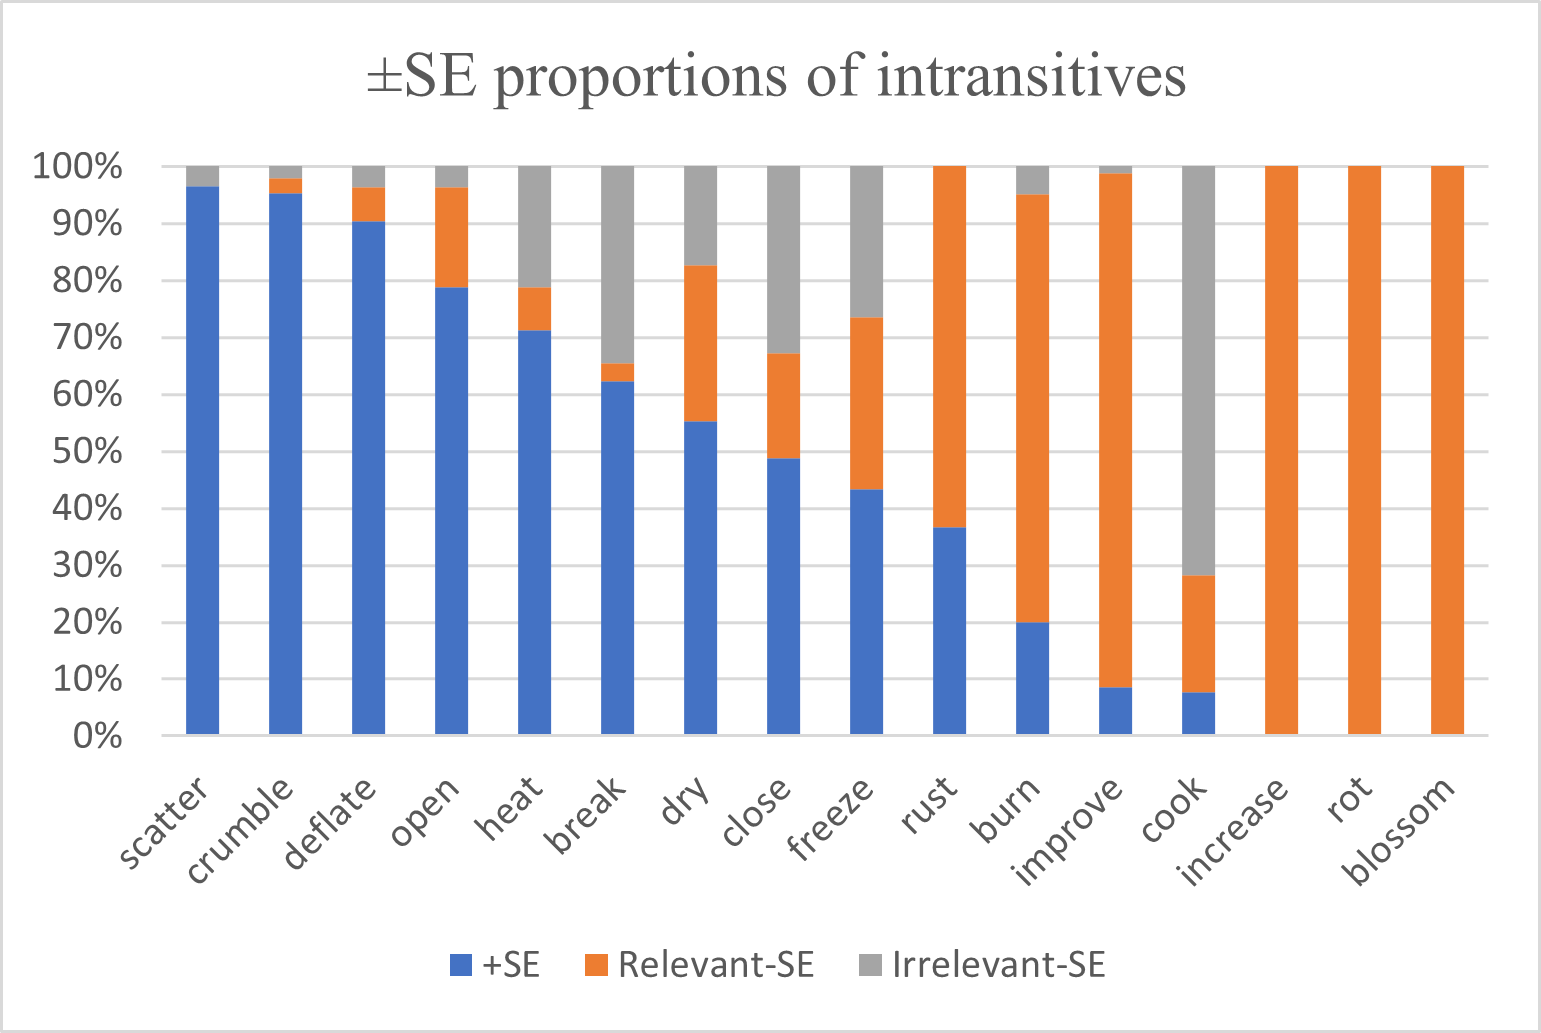
\includegraphics[width=0.8\textwidth]{bentley_figure1.png}
\caption{\label{fig:bentley:figure1}Proportions of +\textsc{se} and -\textsc{se} tokens in the non-passive intransitive subset of each verb}
\end{figure}    

The key result emerging from observation of Figure \ref{fig:bentley:figure1} is that most of the verbs in the sample yielded both +\textsc{se} and relevant -\textsc{se} intransitives. Although the ±\textsc{se} variation was expected with cuocere ‘cook’, \textit{bruciare} ‘burn’, \textit{congelare} ‘freeze’, \textit{sgonfiare} ‘deflate’, \textit{riscaldare} ‘heat’, asciugare ‘dry’, \textit{arrugginire} ‘rust’ (see Table \ref{tab:table1}), it was not expected with \textit{sbriciolare} ‘crumble’, \textit{aprire} ‘open’, \textit{chiudere} ‘close’ and rompere ‘\textit{break}’, which are normally classified as +\textsc{se} verbs, or with \textit{migliorare} ‘improve’, which is classified as -\textsc{se}. In Table 2 we contrast the expected distribution of \textsc{se} with the one recorded in our dataset, highlighting in grey the unexpected results. For completeness, we add the percentages of +\textsc{se} and relevant -\textsc{se} tokens in the non-passive intransitive subset of each verb and the intransitive counts per verb.

\begin{table}[hbt!]
\caption{Intransitive counts of the verbs in the sample and their expected and actual intransitive marking.}
\label{tab:table2}
\begin{tabular}{|p{\textwidth/9}|p{\textwidth/9}||p{\textwidth/9}|p{\textwidth/9}||p{\textwidth/9}|p{\textwidth/9}||p{\textwidth/9}|}
\lsptoprule
Verb (It)    & Verb (En) & Expected intransitive & Actual intransitive marking& \% of \textsc{se} in intransitive subset & \% of relevant -se in intransitive subset & Intransitive counts \\
\midrule
sparpagliare & scatter   & (+ \textsc{se} )                                                                                  & + \textsc{se}                                                                          & 96.6\%                            & 0                                         & 87                  \\
sbriciolare  & crumble   & + \textsc{se}                                                                                     & \cellcolor[HTML]{BFBFBF}± \textsc{se}                                                  & 95.4\%                            & 2.6\%                                     & 153                 \\
aprire       & open      & + \textsc{se}                                                                                     & \cellcolor[HTML]{BFBFBF}± \textsc{se}                                                  & 78.9\%                            & 17.6\%                                    & 143                 \\
chiudere     & clo \textsc{se}      & + \textsc{se}                                                                                     & \cellcolor[HTML]{BFBFBF}± \textsc{se}                                                  & 48.7\%                            & 18.6\%                                    & 156                 \\
rompere      & break     & + \textsc{se}                                                                                     & \cellcolor[HTML]{BFBFBF}± \textsc{se}                                                  & 62.3\%                            & 3.3\%                                     & 151                 \\
cuocere      & cook      & ± \textsc{se}                                                                                     & ± \textsc{se}                                                                          & 7.7\%                             & 20.5\%                                    & 117                 \\
bruciare     & burn      & ± \textsc{se}                                                                                     & ± \textsc{se}                                                                          & 20\%                              & 75.2\%                                    & 145                 \\
congelare    & freeze    & ± \textsc{se}                                                                                     & ± \textsc{se}                                                                          & 43.4\%                            & 30.2\%                                    & 53                  \\
sgonfiare    & deflate   & ± \textsc{se}                                                                                     & ± \textsc{se}                                                                          & 90.4\%                            & 6\%                                       & 301                 \\
riscaldare   & heat      & ± \textsc{se}                                                                                     & ± \textsc{se}                                                                          & 71.3\%                            & 7.5\%                                     & 80                  \\
asciugare    & dry       & ± \textsc{se}                                                                                     & ± \textsc{se}                                                                          & 55.3\%                            & 27.4\%                                    & 179                 \\
arrugginire  & rust      & ± \textsc{se}                                                                                     & ± \textsc{se}                                                                          & 36.6\%                            & 63.4\%                                    & 101                 \\
migliorare   & improve   & - \textsc{se}                                                                                     & \cellcolor[HTML]{BFBFBF}± \textsc{se}                                                  & 8.5\%                             & 90.4\%                                    & 94                  \\
aumentare    & increa \textsc{se}   & - \textsc{se}                                                                                     & - \textsc{se}                                                                          & 0                                 & 100\%                                     & 179                 \\
marcire      & rot       & - \textsc{se}                                                                                     & - \textsc{se}                                                                          & 0                                 & 100\%                                     & 314                 \\
sbocciare    & blossom   & - \textsc{se}                                                                                     & - \textsc{se}                                                                          & 0                                 & 100\%                                     & 350    \\   \lspbottomrule         
\end{tabular}
\end{table}

To be sure, the incidence of \textsc{se} varied considerably, yielding proportions below 10\% with \textit{cuocere} ‘cook’ and \textit{migliorare} ‘improve’ and above 90\% with \textit{sbriciolare} ‘crumble’, \textit{sgonfiare} ‘deflate’, and the sole verb patterning exclusively as +\textsc{se}, namely \textit{sparpagliare} ‘scatter’ (the very few -\textsc{se} tokens of this verb were of the irrelevant type, §3.1). The low \textsc{se} proportions with \textit{cuocere} ‘cook’ depend on the frequent occurrence of this verb in culinary recipes: 71.8\% of the -\textsc{se} non-passive intransitives are irrelevant (cf. 6), while only 20.5\% are anticausatives (see Figure \ref{fig:bentley:figure1} and section 3.1).

As for \textit{migliorare} ‘improve’, despite first appearances it turned out to be a -\textsc{se} verb, in accordance with our expectations (see Table \ref{tab:table1}). Indeed, only one of its +\textsc{se} tokens arguably lent itself to an anticausative analysis (cf. 7a), the others being reflexive, as suggested by the replaceability of atonic \textsc{se} in (7b) with the tonic reflexive sé stesso (... \textit{per migliorare me stesso} ‘to improve myself/my performance’) (§3.1).

\hspace*{\fill}(itTenTen20, 27/11/2022)\quad

\ea
    \ea 
    \gll {Questo studio ha realizzato, col passare degli anni, molti servizi matrimoniali,} specializzandosi e \textbf{migliorandosi} sempre di	più. \\
    {} specialize.\textsc{gerund}.\textsc{se} and improve.\textsc{gerund}.\textsc{se} ever of more\\
    \glt ‘Over the years, this photographic studio has specialized and improved more and more in producing wedding albums.’
    \ex 
    \gll ... continuerò ad impegnarmi al massimo per migliorarmi ... \\
    {} continue.\textsc{fut}.1\textsc{sg}	to do.best.\textsc{inf}.\textsc{se} at.the maximum for improve.\textsc{se} {} \\
    \glt ‘I will continue to do my very best to improve (myself/my performance).’
    \z
\z

Observe also that \textit{migliorare} ‘improve’ occurs in a purposive infinitival clause in (7b) and its missing argument is controlled by a human subject. This indicates intentionality, a facet of meaning which does not pertain to anticausatives but does characterize proper reflexives. Similar considerations were made about the remainder of the +\textsc{se} examples of this verb. 
As for the verbs with high \textsc{se} proportions, the prefix s-, associated with verbs that describe the attainment of a result state \citep[112, 146, 159]{iacobini2004prefissazione}, might at first sight be thought to play a role \textsc{se} marking. However, this hypothesis is challenged by -\textsc{se} \textit{sbocciare} ‘blossom’, which exhibits the same prefix. Therefore, it must be concluded that this morphological feature cannot alone be responsible for \textsc{se} marking. The other unexpected findings, highlighted in grey in Table \ref{tab:table2}, will be discussed in the following sections.  

\subsection{Further Reading}
The following results are of note. First, a subset of the -\textsc{se} verbs participate in the causative alternation, which is not explained by the argument realization analyses (§2). Second, the -\textsc{se} verbs can lexicalize quantized change, while the ±\textsc{se} ones may fail to exhibit \textsc{se} in resultative contexts, which is problematic for the aspectual analyses (§2). Lastly, the rationale of the ±\textsc{se} variation is not the same with all verbs and reveals a contrast between two subclasses of verbs. 
This contrast will turn out to correlate with the selection of different perfect auxiliaries in the -\textsc{se} intransitives, a fact which has not yet received due attention (though see \cite{bentley2021two}). We shall discuss these issues in turn.

\subsubsection{Alternating -\textsc{se} verbs}
The existence of alternating verbs which never exhibit \textsc{se} in the intransitive is not a novel result (§1). The purpose of this section is to identify which verbs from our sample belong in this group and to discuss the properties which set them apart from the alternating verbs that admit \textsc{se} marking. In Figure \ref{fig:bentley:figure2} we show the proportions of transitive hits obtained for each verb.

\begin{figure}[hbt!]
\centering
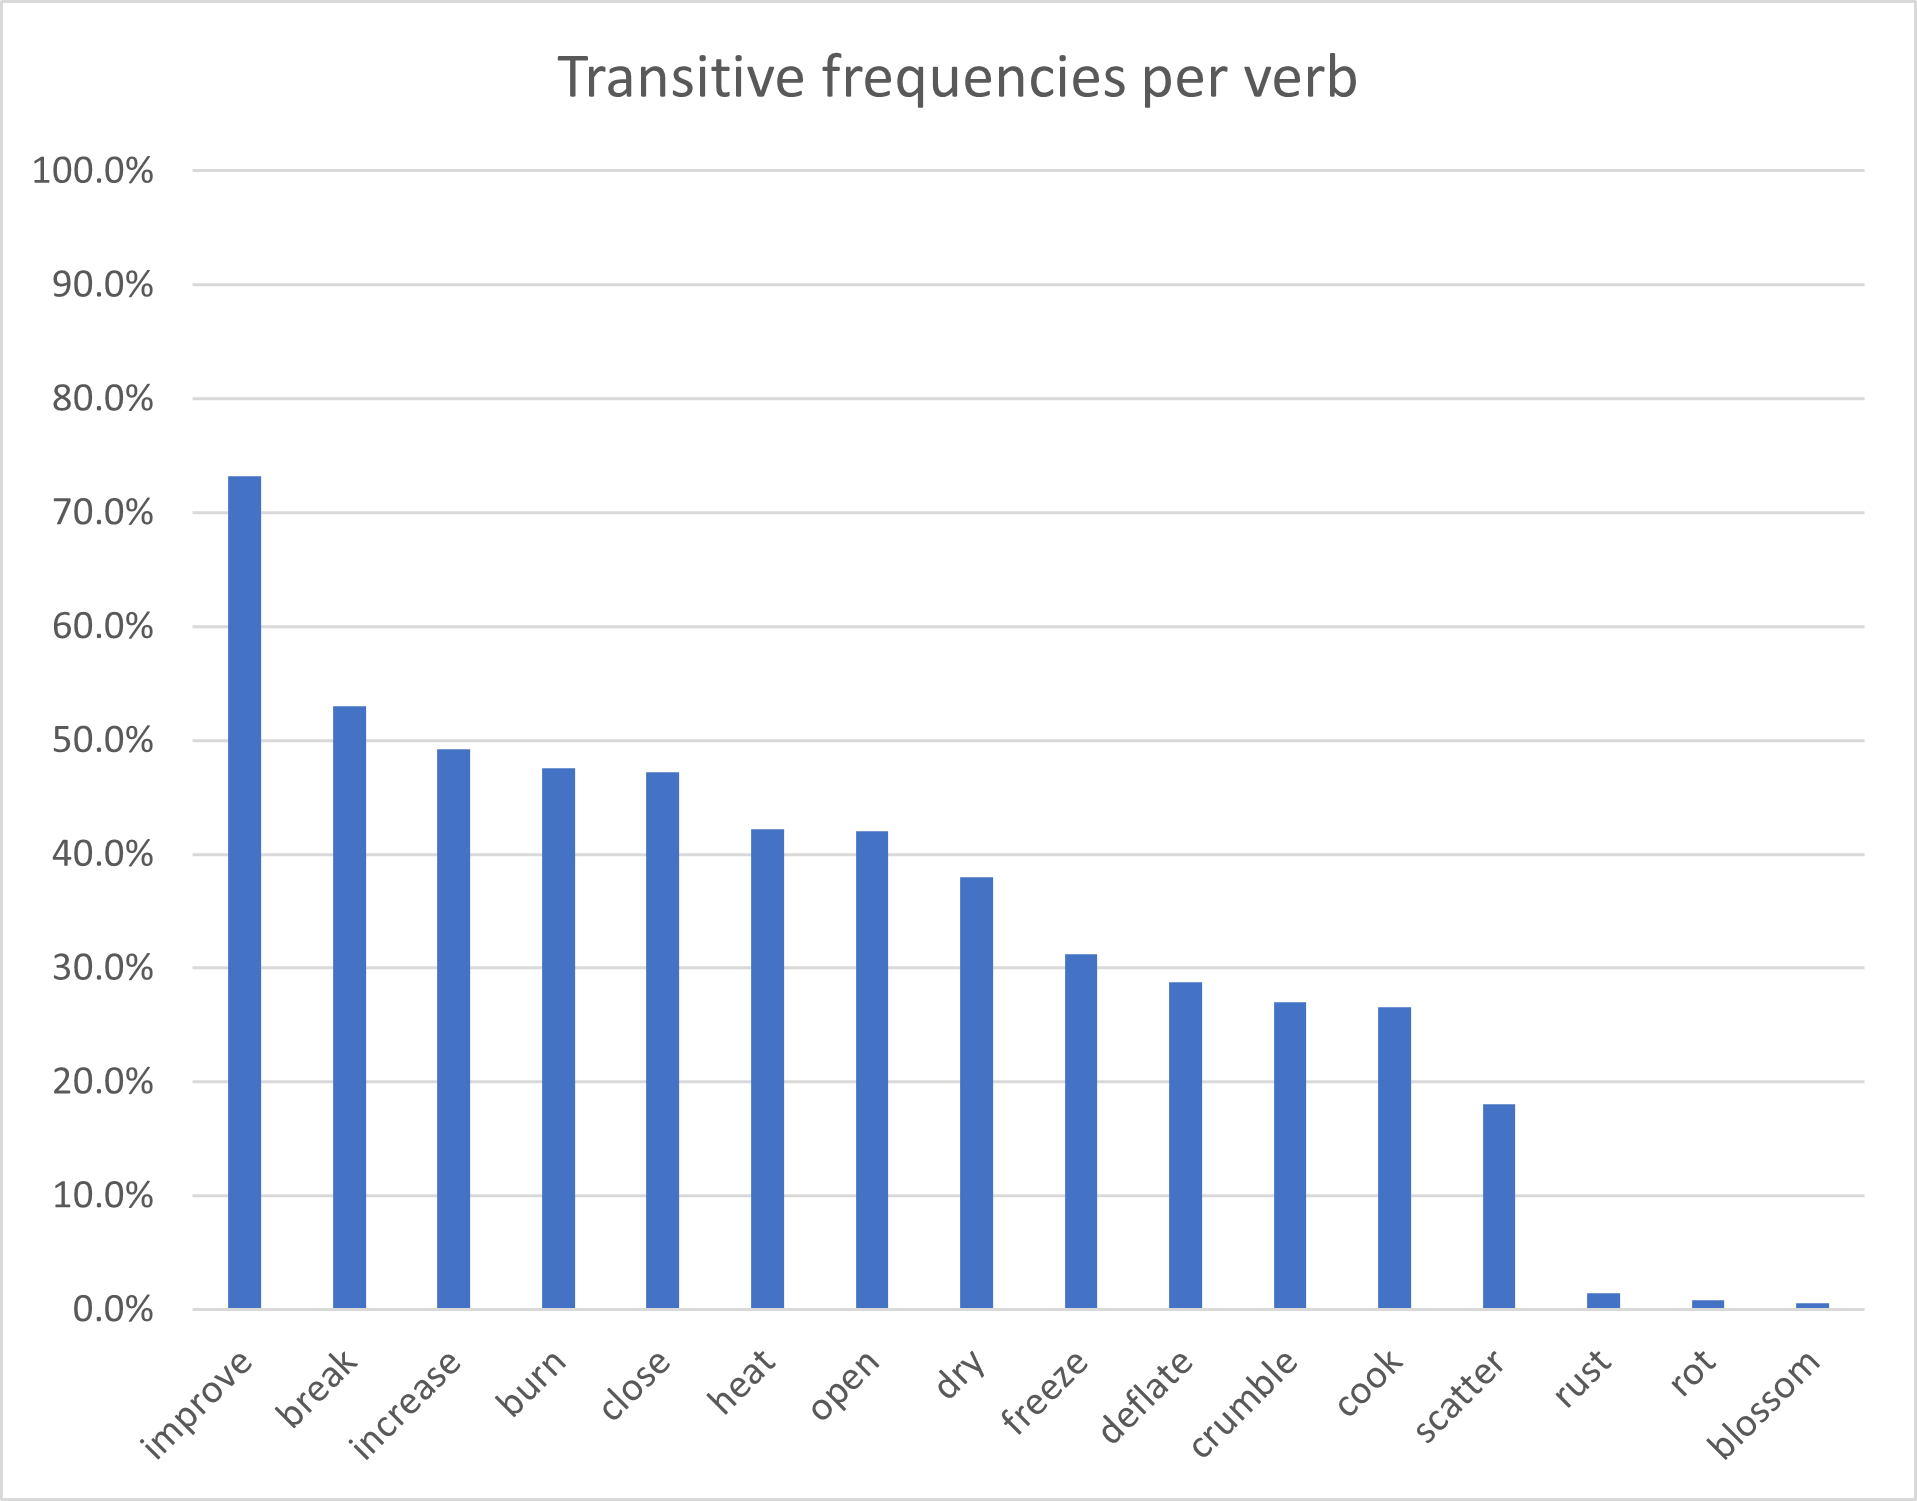
\includegraphics[width=0.8\textwidth]{bentley_figure2.png}
\caption{\label{fig:bentley:figure2}Proportions of transitive attestations }
\end{figure}    

Observation of Table \ref{tab:table2} and Figure \ref{fig:bentley:figure2} suggests that \textit{aumentare} ‘increase’ is an alternating   -\textsc{se} verb. We provide an intransitive and, respectively, a transitive example of this verb here.

\hspace*{\fill}(itTenTen20, 29/10/2022)\quad

\ea
    \gll ... i casi di tumore del pancreas sono \textbf{aumentati} del 59\% ... \\
    {} the cases of tumour of.the pancreas be.3\textsc{pl} increase.\textsc{ptcp} of.the 59\% {} \\
    \glt ‘The incidence of pancreatic cancer has increased by 59\%...’
\z

\ea
    \gll [L]a	crisi		economica	avrebbe 							\textbf{aumentato}  \\
    the		crisis	economic		have.\textsc{cond}.3\textsc{sg}	increase.\textsc{ptcp}\\
    \glt ‘The economic crisis would increase the incidence of age discrimination.’
\z

The intransitive example illustrates the absence of \textsc{se} marking, which is exceptionless with this verb in our dataset. As for the transitive example, the fact that the higher argument (\textit{la crisi economica} ‘economic crisis’) is inanimate supports a causative – as opposed to agentive - analysis. This is further corroborated by the possibility of paraphrasing this structure with a causative periphrasis \citep[26-27 and references therein]{zribi1987reflexivite}.

\ea
    \gll La	crisi		economica	avrebbe 							\textbf{fatto} \textbf{aumentare} {l’incidenza...}\\
    				the	crisis	economic		have.\textsc{cond}.3\textsc{sg}	make.\textsc{ptcp}	increase.\textsc{inf}	the incidence\\
    \glt  	‘The economic crisis would increase the incidence of age discrimination.’
\z

Non-causative agentive verbs are not synonymous with their causative periphrastic counterparts, as shown by the different meanings of the authentic example in (11a) and its constructed counterpart in (11b): an agent, and not the \textit{fare} ‘make’ causer, is understood to be the higher argument of the embedded infinitive in (11b).

\hspace*{\fill}(itTenTen20, 09/06/2023)\quad

\ea
    \ea 
    \gll In	due	giorni	ho						\textbf{ricamato}						un cuscinetto... \\
    in	two	days			have.1\textsc{sg}	embroider.\textsc{ptcp}	a			cushion.\textsc{diminutive}\\
    \glt ‘I embroidered a small cushion in two days.’
    \ex 
    \gll In	due	giorni	ho						\textbf{fatto}						\textbf{ricamare}					un	cuscinetto... \\
   	in	two	days			have.1\textsc{sg}	made.\textsc{ptcp}	embroider.\textsc{inf}		a			cushion.\textsc{diminutive} \\
    \glt ‘I had someone embroider a small cushion in two days.’
    \z
\z

The contrast between \textit{aumentare} ‘increase’ and \textit{ricamare} ‘embroider’ supports the hypothesis that the transitive of the former verb is a causative structure. Thus, this verb participates in the causative alternation. 
\textit{Migliorare} ‘improve’ can also be classified as an alternating -\textsc{se} verb, despite the findings reported in Table \ref{tab:table2}, because its \textsc{se} marked intransitive tokens are mostly reflexive (§3.2, cf. 7b). We should also note that this verb has the highest transitive percentages (see Figure \ref{fig:bentley:figure2}) and the transitive tokens pass the causativity test mentioned above, as suggested by the synonymity of (12a) with its constructed paraphrase in (12b).

\ea
    \ea 
    \gll 	Il		divieto		di		fumo		ha							migliorato				la		salute		dei				baristi... \\
    						the	ban				of		smoke	have.3\textsc{sg}		improve.\textsc{ptcp}		the	health	of.the		bartenders				\\
    \ex 
    \gll In		Il		divieto		di		fumo		ha							fatto						migliorare 	la 	salute 	dei			 baristi \\
   	the	ban				of		smoke	have.3\textsc{sg}		make.\textsc{ptcp}	improve.\textsc{inf}	the	health	of.the		bartenders \\
    \glt 					‘The ban on smoking has improved the health of bartenders.’
    \z
\z

In Table \ref{tab:table3} we show the results on transitivity and anticausative marking, highlighting the two alternating -\textsc{se} verbs. (In the next section, we shall explain why the other -\textsc{se} verbs, \textit{marcire} ‘rot’ and \textit{sbocciare} ‘blossom’, are classified as -transitive.)

\begin{table}[hbt!]
\caption{±Transitive vis-à-vis ±\textsc{se} behaviour: the alternating -\textsc{se} verbs}
\label{tab:table3}
\begin{tabular}{llll}
\lsptoprule
Verb (It)    & Verb (En) & Transitive & Anticausative marking \\
\midrule
\textit{sparpagliare} & scatter   & +          & +se   \\
\textit{sbriciolare}  & crumble   & +          & ±se   \\
\textit{aprire}       & open      & +          & ±se   \\
\textit{chiudere}     & close     & +          & ±se   \\
\textit{rompere}      & break     & +          & ±se   \\
\textit{cuocere}      & cook      & +          & ±se   \\
\textit{bruciare}     & burn      & +          & ±se   \\
\textit{congelare}    & freeze    & +          & ±se   \\
\textit{sgonfiare}    & deflate   & +          & ±se   \\
\textit{riscaldare}   & heat      & +          & ±se   \\
\textit{asciugare}    & dry       & +          & ±se   \\
\textit{arrugginire}  & rust      & +          & ±se   \\
\textit{migliorare}   & improve   & +          & \textbf{-se}   \\
\textit{aumentare}    & increase  & +          & \textbf{-se}   \\
\textit{marcire}      & rot       & -          & -se   \\
\textit{sbocciare}    & blossom   & -          & -se   \\              
\lspbottomrule
\end{tabular}
\end{table}

Having ascertained that both \textit{aumentare} ‘increase’ and \textit{migliorare} ‘improve’ belong in the alternating -\textsc{se} class, we can explore the properties that differentiate them from the alternating verbs that admit \textsc{se} marking. Previous accounts have relied on lexical aspect or a loose principle of spontaneity (§§1-2). A problem with the idea that alternating verbs do not take \textsc{se} if they are degree achievements is that many ±\textsc{se} alternating verbs (\textit{cuocere} ‘cook’, \textit{asciugare} ‘dry’, \textit{congelare} ‘freeze’, \textit{bruciare} ‘burn’, \textit{sgonfiare} ‘deflate’, \textit{riscaldare} ‘heat’, etc.) are also degree achievements, as suggested by the application of the relevant tests \citep{dowty1979word,bertinetto1995attempt,hay1999scalar}. Among such diagnostics are the entailment of the perfect by the progressive; the compatibility with expressions of measure like ‘a lot’ and with both ‘in’ and ‘for’ temporal adverbials; the fact that when the verb combines with ‘almost’, two readings are obtained: according to the one, the event has occurred but has not been completed; according to the other, the event has not occurred at all. The context can coerce the one or the other reading (for aspectual coercion see \cite{jackendoff1997architecture}: 51-53, \cite{jackendoff2002foundations}: 290-292; \cite{pustejovsky1991syntax}) shall leave it for the reader to apply the tests by themselves. Here we should point out that the property of being a degree achievement cannot be the \textit{explanans} of the absence of \textsc{se} with the alternating -\textsc{se} verbs since it does not pick out this subclass alone. 

As for spontaneity, while increasing and improving may occur more spontaneously than heating and cooking, the consideration of other alternating -\textsc{se} verbs of Italian does not support the hypothesis that spontaneity is the key factor in the absence of \textsc{se} marking with these verbs. Alongside the antonyms of \textit{aumentare} ‘increase’ and \textit{migliorare} ‘improve’, \textit{diminuire} ‘decrease’ and \textit{peggiorare} ‘worsen’, the literature cites \textit{affondare} ‘drown/sink’, \textit{cambiare} ‘change’, \textit{guarire} ‘heal’, \textit{crescere} ‘grow’, and \textit{bollire} ‘boil’ as alternating -\textsc{se} verbs. It is hard to see why boiling events should be more spontaneous than heating events, and so on.

In an analysis of Romance verbs of internal causation (in the sense of \cite{levin1995unaccusativity}), we argued that the alternating -\textsc{se} subset of such verbs describes events which do not fully satisfy \citet[4-5]{wolff2003direct} conditions on direct causation. According to this author, causation is direct if:


\ea
    \ea 
    \glt There are no intervening entities at the same level of granularity as initial causer and final causee 	OR  \\
    \ex 
    \glt Any intervening entity is construable as an enabling condition rather than a cause.  \\
    \z
\z

The alternating -\textsc{se} verbs of internal causation describe events which can have multiple causes at the same level of granularity \citep{bentley2023internally}. A prime example is that of ‘ferment’ verbs, which can describe events caused by humans relying on the intervention of organisms such as yeast and bacteria. Without such organisms the change cannot occur, and, in fact, yeast and bacteria can cause the change by themselves. Thus, these interveners are not optional enabling conditions, but rather causes in their own right. 

The alternating -\textsc{se} verbs listed above can also describe complex causation chains with indirect causes and necessary interveners, which alone cause the relevant changes. Think of the role of seawater in the sinking of a ship or heated water in the boiling of an egg and contrast these roles with the participation of a key in the opening of a door or a hammer in the smashing of a chair. The last two are optional instruments, which enable the causer to achieve their goal. The first two are not: they cannot be dispensed with and, in fact, they are the true causes of the change (even when the ship has been scuppered and the egg has been put on the hob). To return to the alternating -\textsc{se} verbs in our sample, economic crises are not the immediate cause of age discrimination (cf. 9), but they can have such discrimination among their ultimate consequences if they result in poorer job offer or similar intervening scenarios, which will involve discriminators. Similarly, the ban on smoking results in the bartenders’ reduced exposure to smoke, which in turn will reduce the likelihood of bartenders contracting smoke-related ailments (cf. 12a). Of course, it could be argued that these events occur at different levels of granularity. The key issue, however, is that with these verbs the level of granularity is irrelevant to the encoding of causation chains. As \citet[477]{kiparsky1997remarks} puts it, “there is no question that the boundaries of direct causation are fuzzy." Alternating -\textsc{se} verbs in Italian provide a clear illustration of this fuzziness, while also suggesting that indirect causation can be encoded in the lexicon. Key evidence that it is this property that underlies the lack of \textsc{se} is provided by pairs such as -\textsc{se} \textit{cambiare} ‘change’ and its +\textsc{se} counterpart \textit{cambiarsi}. The latter only means ‘to change one’s clothes or one facial expression’ (https://www.treccani.it/vocabolario/cambiare/), these being changes which do not require or admit interveners. +\textsc{se} \textit{cambiarsi} thus describes direct causation, unlike -\textsc{se} \textit{cambiare}. 

In section 5.4.1 we shall argue that a constructional constraint rules out \textsc{se} anticausativization in Italian, when the conditions on direct causation are not satisfied. In this perspective, the verbs discussed here do not challenge the argument realization analyses of \textsc{se} anticausativization, after all.

\subsubsection{-\textsc{se} verbs of quantized change and resultative -\textsc{se} constructions}

The other -\textsc{se} verbs in our sample were marcire ‘rot’ and sbocciare ‘blossom’ (see Chart 1), exemplified below.

\hspace*{\fill}(itTenTen20, 25/08/2022)\quad
\ea
    \gll {... la		tettoia ...	l’	hanno fatta in bambù} 
    ed		\textbf{è} 					\textbf{marcita}	in	una	stagione.  \\
 {} 				and	be.3\textsc{sg}	rot.\textsc{ptcp}		in	one	season \\
    \glt 			‘The roof ... they made it with bamboo and it rotted away in one season.’
\z



\hspace*{\fill}(itTenTen20, 12/06/2023)\quad

\ea
    \gll I			fiori				vengono		\textbf{sbocciano}				ed		appassiscono	in 	una sola			giornata. \\
 the	flowers	come.3\textsc{pl}		blossom.3\textsc{pl}	and	wither.3\textsc{pl}				in		one	single	day \\
    \glt 				‘The flowers come, blossom and wither in a single day.’
\z

Unlike \textit{aumentare} ‘increase’ and \textit{migliorare} ‘improve’, \textit{marcire} ‘rot’ and \textit{sbocciare} ‘blossom’ were classified as non-transitivizing because their transitive hits amounted to less than 1\% of their overall attestations (see Appendix 2). These results are highlighted in Table \ref{tab:table4}.

\begin{table}[hbt!]
\caption{±Transitive vis-à-vis ±\textsc{se} behaviour: the non-alternating -\textsc{se} verbs}
\label{tab:table4}\begin{tabular}{llll}
\lsptoprule
Verb (It)    & Verb (En) & Transitive & Anticausative marking \\
\midrule
sparpagliare & scatter   & +          & +se                   \\
sbriciolare  & crumble   & +          & ±se                   \\
aprire       & open      & +          & ±se                   \\
chiudere     & close     & +          & ±se                   \\
rompere      & break     & +          & ±se                   \\
cuocere      & cook      & +          & ±se                   \\
bruciare     & burn      & +          & ±se                   \\
congelare    & freeze    & +          & ±se                   \\
sgonfiare    & deflate   & +          & ±se                   \\
riscaldare   & heat      & +          & ±se                   \\
asciugare    & dry       & +          & ±se                   \\
arrugginire  & rust      & +          & ±se                   \\
migliorare   & improve   & +          & -se                   \\
aumentare    & increase  & +          & -se                   \\
marcire      & rot       & -          & \textbf{-se}          \\
sbocciare    & blossom   & -          & \textbf{-se}           \\
\lspbottomrule
\end{tabular}
\end{table}

We should also mention that the few transitive tokens of these verbs have figurative meanings (cf. 16), i.e., do not describe change in the physical world, or non-conventional meanings (cf. 17), which are not reported in dictionaries and are deemed to be unacceptable by native speakers\footnote{Drawing on \citet{mcnally2022grammatically}, we assume that the grammatically relevant aspects of the meaning of a verb can be carried over to its figurative extensions. Therefore, the evidence in (16) is relevant to the causative alternation, although there is very little of it. We found no evidence of literal \textit{marcire} ‘rot’ used transitively. }.

\hspace*{\fill}(itTenTen20, 25/08/2022)\quad
\ea
    \gll {... il malcostume ...  abbia guastato e} \textbf{marcito}	la			questione	meridionale...  \\
    {} rot.\textsc{ptcp}		the		issue					southern \\
    \glt ‘... corruption has ruined and rotted the issue of the South.’
\z


\hspace*{\fill}(itTenTen20, 25/08/2022)\quad
\ea
    \gll Chiaro 			senza			\textbf{sbocciare} bottiglie	in	discoteca		ogni		sera  \\
 of.course		without	\textit{sbocciare}	bottles			in disco					every evening \\
    \glt ‘Of course, without opening (?) bottles in the disco every evening.’
\z

\textit{Sbocciare} ‘blossom’ was also unattested in the passive, whereas \textit{marcire} ‘rot’ yielded four passive tokens (<1\% of its overall attestations), one of which translates as ‘rust’ rather than ‘rot’. Overall, the evidence does not support a causative analysis of these verbs, although as was suggested in our study of verbs of internal causation \citep{bentley2023internally}, \textit{marcire} ‘rot’ may have a causative realization in some varieties of Italian.

The two verbs under discussion provide important evidence because they suggest that neither the lexicalization of quantized change nor the resultativity of a construction can alone explain the occurrence of \textsc{se}. We shall begin by noting that neither verb takes \textsc{se} when modified by an ‘in’ temporal adverbial, as can be seen in (14) and (15). Assuming such adverbials coerce a resultative reading (\cites[332-336]{dowty1979word}{hay1999scalar}) these are examples of resultative constructions that lack \textsc{se} marking.

As for lexical aspect, both verbs are attested as participial adjectives, which indicates that they lexicalize a result state of some sort (\cites[]{hout2004unaccusativity}[355]{bentley2006split}[283-284]{legendre2017auxiliaries}). Relevant percentages are given in Appendix 2.

\hspace*{\fill}(itTenTen20, 25/08/2022)\quad
\ea
    \gll tubature		\textbf{marcite}					da 	sostituire.   \\
    pipe.\textsc{fpl}	rot.\textsc{ptcp}.\textsc{fpl}	to		replace.\textsc{inf}		 \\
    \glt ‘rotten pipes to be replaced.’
\z


\hspace*{\fill}(itTenTen20, 25/08/2022)\quad
\ea
    \gll un	piccolo	fiore						\textbf{sbocciato}   \\
    a			small			flower.\textsc{msg}	blossom.\textsc{ptcp}.\textsc{msg}	 \\
    \glt ‘a small, blossomed, flower.’
\z

However, \textit{marcire} ‘rot’ tests out as a degree achievement and is thus unproblematic for the aspectual hypothesis or a version thereof. Instead, \textit{sbocciare} ‘blossom’ does not combine with expressions of measure or with ‘for’ temporal adverbials, nor does its progressive entail the perfect. Since this verb was attested in the progressive and in combination with ‘begin’, ‘finish’ and the adverb ‘completely’, we shall tentatively analyse it as an accomplishment. Further investigation may reveal an achievement analysis to be more fitting\footnote{In combination with ‘almost’, sbocciare ‘blossom’ seems to us to yield a counterfactual reading, which suggests that it might be an achievement \citep{hay1999scalar}}.  However, what matters in the present context is that this verb lexicalizes quantized change and fails to take \textsc{se}. 

In sum, the behaviour of the non-alternating -\textsc{se} verbs suggests that neither the lexicalization of a specific result state nor the occurrence in a construction that coerces resultativity are sufficient conditions for \textsc{se} marking in the absence of causation (a point previously made by \citet{jimenez2017causativity} with reference to Southern Peninsular Spanish).  

\subsubsection{Principles underlying the ±\textsc{se} variation}

Turning now to the verbs which exhibited variation in the marking with anticausative \textsc{se}, the evidence suggests that different principles underlie the -\textsc{se} realization of different subclasses of such verbs. With one subclass, only comprising degree achievements, the absence of \textsc{se} loosely correlates with the description of properties or processes. Instead, the -\textsc{se} realization of the other subclass is underpinned by indirect causation. This latter subclass includes accomplishment verbs, which have so far been labelled as +\textsc{se} in the literature. The verbs of the first subclass may also fail to exhibit \textsc{se} when the cause is not direct, whereas the verbs of the second subclass never fail to exhibit \textsc{se} when describing properties. The remaining cases of ±\textsc{se} variation will be subsumed under the label of polysemy. In section 4 we discuss these findings in depth.

\section{The ±\textsc{se} variation}
\subsection{Absence of \textsc{se}: properties and processes}
Scrutiny of the verbs which are known from the literature to exhibit ±\textsc{se} variation (see Tables \ref{tab:table1} and \ref{tab:table2}) reveals that the -\textsc{se} intransitives of these verbs can describe properties or processes. The cause is irrelevant in property descriptions because what is at issue is a feature of the causee. 

\hspace*{\fill}(itTenTen20, 23/08/2022)\quad
\ea
    \gll \textbf{Cuociono} e			si		sfaldano		lentamente (come tutti i legumi della stessa consistenza.)    \\
    cook.3\textsc{pl}		and	\textsc{se}		flake.3\textsc{pl}		slowly {}\\
    \glt ‘[Yellow split peas] cook and flake slowly like all pulses with the same texture.’
\z

\hspace*{\fill}(itTenTen20, 30/08/2022)\quad
\ea
    \gll Realizzato	in una microfibra		leggera,	che			asciuga		rapidamente. \\
    make.\textsc{ptcp}	in	a				microfiber		light				\textsc{rel}		dry.3\textsc{sg}		quickly \\
    \glt ‘Made in a light microfiber, which dries quickly.’
\z

\hspace*{\fill}(itTenTen20, 02/09/2022)\quad
\ea
    \gll I tuberi \textbf{congelano} a -2ºC.\\
    	the		bulbs		freeze.3\textsc{pl}		at		-2ºC \\
    \glt ‘The bulbs freeze at -2ºC.’
\z


The lack of a specific time reference and the occurrence of manner adverbials are hallmarks of the construction that is sometimes referred to as ‘facilitative’ \citep[147-149]{kemmer1993middle} (see also \cite[25-26]{levin1993english}). \textsc{se} is not ruled out from this construction, as evidenced by an example with a verb from the putatively +\textsc{se} subclass.


\hspace*{\fill}(itTenTen20, 02/09/2022)\quad
\ea
    \gll ... le		chiome risultano				secche,	asciutte e				si 		rompono facilmente.\\
    	{} 								the	hair				become.3\textsc{pl}	dry					dry					and	\textsc{se}		break.3\textsc{pl}	easily \\
    \glt ‘Hair becomes dry and breaks easily.’ 
\z

Therefore, the absence of \textsc{se} in (20)-(22) cannot be the spell-out of a property description construction. Instead, let us temporarily assume that it is a strategy that leaves out irrelevant facets of verb meaning, namely the cause. 
The -\textsc{se} intransitives of the verbs that are normally labelled as ±\textsc{se} can also describe the unfolding of events of change of state. 

\ea
    \underline{Description of processes} 
    \ea 
    \gll Mentre	le			uova	\textbf{cuociono}, { prepariamo la salsa olandese. (itTenTen20, 23/08/2022)} \\
    while			the		eggs		cook.3\textsc{pl} {} \\
    \glt ‘While the eggs are cooking, we make the hollandaise sauce.’ \\
    \ex
    \gll ... lo chassis ... che		già 				\textbf{sta} 			\textbf{asciugando}	in 	terrazzo. {(itTenTen20, 30/08/2022)}\\
    {} the	chassis	 {}				\textsc{rel}	already	be.3\textsc{sg}	dry.\textsc{gerund}	in		balcony	{} \\
    \glt 	‘The chassis which is already drying on the balcony.’ \\
    \ex
    \gll Infilare			nel			Freezer	a		\textbf{congelare}		per 	una	mezzoretta. {(itTenTen20, 02/09/2022)}\\
    put.in.\textsc{inf}		in.the	freezer		at	freeze.\textsc{inf}	for		one	half.hour.\textsc{diminutive}	{} \\
    \glt 					‘Put it in the freezer (to freeze) for half an hour.’ \\
    \z
\z

Similar considerations can be made for \textbf{bruciare} ‘burn’, \textbf{sgonfiare} ‘deflate’ and \textbf{riscaldare} ‘heat’, although for brevity we shall not provide any exemplification here. 
The evidence in (24) contrasts with that in (25), where what is being described is change leading to meat rolls being cooked, hair being dry, and mammoths being frozen. In this case the verb is marked with \textsc{se}.

\ea
    \underline{Descriptions of change leading to result state} 
    \ea 
    \gll Dopo che	si 		\textbf{sono} 		\textbf{cotti}, ... tagliarli			a fettine. {(itTenTen20, 23/08/2022)} \\
   				after		that	\textsc{se}		be.3\textsc{pl}	cook.\textsc{ptcp}	{} slice.them	to	slices.\textsc{diminutive} {} \\
    \glt ‘After they [meat rolls] have cooked, slice thinly.’ \\
    \ex
    \gll Quando		i		capelli	si		\textbf{sono} 		\textbf{asciugati} ... appaiono		come “incollati”. {(itTenTen20, 30/08/2022)}\\
    when			the	hair			\textsc{se}		be.3\textsc{pl}	dry.\textsc{ptcp}	{}					seem.3\textsc{pl}		like			glued	{} \\
    \glt 					‘When the hair has dried, it will seem glued together.’ \\
    \ex
    \gll ... i			mammut,		mentre		mangiavano ... si 		\textbf{sono} 		\textbf{congelati} 		all’istante. {(itTenTen20, 02/09/2022)} \\
    {} 									the	mammoths	while			eat.\textsc{pst}.3\textsc{pl}			{}			\textsc{se}		be.3\textsc{pl}	freeze.\textsc{ptcp}	 at.the.instant	{} \\
    \glt 									‘While the mammoths	 were eating, they froze instantly.’ \\
    \z
\z

We note that the -\textsc{se} intransitives are not incompatible with expressions that coerce the notion of a result state being attained (cf. 26), while the +\textsc{se} ones can also describe the unfolding of events of change (cf. 27-28).

\hspace*{\fill}(itTenTen20, 23/08/2022)\quad
\ea
    \gll È	pasta	fresca,	quindi \textbf{cuocerà} 					\textit{nell}’			\textit{arco}		\textit{di}	 	\textit{pochi} \textit{minuti}. \\
    		is	pasta	fresh		so					cook.\textsc{fut}.3\textsc{sg}	in.the		arch		of		few		minutes \\
    \glt ‘It is fresh pasta, so it will cook in a couple of minutes.’
\z

\hspace*{\fill}(itTenTen20, 30/08/2022)\quad
\ea
    \gll {Bisogna riportare il disegno ... e lasciare}  che		\textbf{si}		\textbf{asciughi}					\textit{per}		\textit{circa}	2	\textit{giorni}. \\
    	{} 		that	\textsc{se}		dry.\textsc{sbjv}.3\textsc{sg}		for		circa	2	days \\
    \glt	‘One needs to take the drawing back… and let it dry for about two days.’
\z

\hspace*{\fill}(itTenTen20, 02/09/2022)\quad
\ea
    \gll \textit{Mentre}	l’		acqua		\textbf{si}		\textbf{congela},			si		espanderà {	allargando la pelle nel processo...}\\
    	as						the	water		\textsc{se}		freeze.3\textsc{sg}		\textsc{se}		expand.\textsc{fut}.3\textsc{sg} {} \\
    \glt 	‘As the water freezes, it will expand, extending the skin in the process.’
\z

Example (26) shows that ‘in’ temporal adverbials do not necessarily trigger \textsc{se} marking, while the following examples indicate that the description of duration rather than completion is not incompatible with \textsc{se} marking: see the ‘for’ temporal adverbial in (27) and the temporal subordinator \textit{mentre} ‘as/while’, as well as the reference to a process, in (28). 

Overall, the evidence jars with the analysis of \textsc{se} as the spell-out of a resultative construction, i.e., a construction that provides a resultative meaning component. However, it does not rule out the hypothesis that a facet of the meaning of the relevant verbs underpins the general tendencies mentioned above. Application of the diagnostics mentioned in section 3.3.1 reveals \textit{cuocere} ‘cook’, \textit{asciugare} ‘dry’, \textit{congelare} ‘freeze’, \textit{bruciare} ‘burn’, \textit{sgonfiare} ‘deflate’ and \textit{riscaldare} ‘heat’ to be degree achievements. We noted that lexical aspect, and in particular the properties of degree achievements, cannot alone explain the distribution of \textsc{se}. Nonetheless, these properties turn out to have a bearing on the ±\textsc{se} variation described in this section. 

\subsection{Absence of \textsc{se}: indirect causation}

The -\textsc{se} attestations of \textit{chiudere} ‘close’, \textit{aprire} ‘open’, \textit{rompere} ‘break’ and \textit{sbriciolare} ‘crumble’ do not describe properties or processes, as is suggested by perfect aspect in (29)-(31) and the temporal adverbials indicating when the change has been or will be completed in (29), (30) and (32).

\hspace*{\fill}(itTenTen20, 15/01/2023)\quad
\ea
    \gll I			seggi										\textbf{hanno}			\textbf{chiuso} 				ieri 						sera 		\textit{alle}		22. \\
    the	polling.stations	have.3\textsc{pl}	close.\textsc{ptcp}		yesterday	night	at.the	10 \\
    \glt 	‘The polling stations closed at 10pm last night.’
\z

\hspace*{\fill}(itTenTen20, 31/10/2022)\quad
\ea
    \gll La		casa			\textbf{ha}						\textbf{aperto}				4	\textit{mesi}				\textit{fa}, {però il lavoro con la comunità è iniziato prima.}\\
    			the		home		have.3sg	open.ptcp	4	months	ago {} \\
    \glt 				‘The home opened four months ago, but the work of the community began before then.’
\z

\hspace*{\fill}(itTenTen20, 27/11/2022)\quad
\ea
    \gll {Giaceva sul letto e la struttura del letto} \textbf{ha}						\textbf{rotto}						a		tutti	e				quattro 	gli 	angoli.  \\
    	{} 	have.3\textsc{sg}	break.\textsc{ptcp}	at	all		and	four				the	corners\\
    \glt 				‘He was lying on the bed and the frame of the bed broke at all four corners.’
\z

\hspace*{\fill}(itTenTen20, 31/08/2022)\quad
\ea
    \gll Entro		\textit{massimo}			\textit{due}	\textit{anni}		\textbf{sbriciolerà}. \\
    	within	maximum		two	years	crumble.\textsc{fut}.3\textsc{sg} \\
    \glt 				‘Within two years it will crumble.’
\z

A clue to understand the absence of \textsc{se} with these verbs is provided by the observation that these -\textsc{se} intransitives are incompatible with the addition \textit{da sé/da solo} ‘by itself’ in the sense of ‘without outside help’. Since \citet{chierchia1989semantics} this adverbial has been cited as a causative diagnostic. \citet[76-79]{alexiadou2015external}  claim that\textit{ da sé/da solo} ‘by itself’ does not identify a causer, but rather rejects the participation of a causer in the event. Since the verbs under discussion participate in the causative alternation, they should readily combine with ‘by itself’. Indeed, they do, when \textsc{se} marked.

\hspace*{\fill}(itTenTen20, 17/01/2022)\quad
\ea
    \ea
    \gll {Mi sono solo avvicinato alla maniglia} 	e				la		porta	\textbf{si}		\textbf{è}							\textbf{aperta}				\textbf{da} \textbf{sola}.	\\
    {} and	the	door		\textsc{se}		be.3\textsc{sg}		open.\textsc{ptcp}	by	alone \\
    \glt 					‘I simply approached the handle and the door opened by itself.’
    \ex
    \gll Dopo		due	mesi			la		ferita			\textbf{si} 		\textbf{è }						\textbf{chiusa} 			\textbf{da} \textbf{sola}. \\
				after			two	months	the	wound		\textsc{se}		be.3\textsc{sg}		close.\textsc{ptcp}	by	alone\\
    \glt 				‘After two months the wound closed by itself.’
    \z
\z

An effect of the rejection of the participation of the causer is that it strengthens an inference of responsibility on the part of the causee, which arises with \textsc{se} marking (\cites[and references therein]{zribi1987reflexivite}[]{kailuweit2012construcciones}[see section 5.4.1 for further discussion]{martin2014anticausatives}). This inference is irreconcilable with the construction discussed in this section because this gives rise to another inference, i.e., that any direct cause is irrelevant and there may be a remote cause. Example (29) is about the time when it was no longer possible to exercise the right to vote: the closing, and closers, of the physical doors of the polling stations are irrelevant. Similarly, example (30) does not describe the physical opening of the doors of a house, but rather makes the point that the community under discussion has had a home for four months. In (31) the implication is that the bed must have been faulty and, therefore, the cause of its breaking, presumably the manufacturers, is more remote than the person who lay on it and the bed itself. Lastly, (32) is part of a complaint for inaction and lack of maintenance, which is likely to result in the crumbling of a building: there is no physical “crumbler” in this event, nor is the building itself responsible for the crumbling.

The addition of\textit{ da sé/da solo} ‘by itself’ is non-sensical in concomitance with the perfect auxiliary \textit{avere} ‘have’, which characterizes the -\textsc{se} pattern under discussion here (cf. 29-31), because ‘by itself’ and the {-\textsc{se}, +perfect ‘have’} pattern trigger contradictory inferences: responsibility of the causee and, respectively, indirect causation and irrelevance of any direct cause. We should note that verbs of change of state are expected to select \textit{essere} ‘be’ in the perfect in Italian (cf. 8, 14 and see \cite{perlmutter1989multiattachment} and the subsequent literature on the semantic parameters of perfect auxiliary selection). Therefore, the selection of \textit{avere }‘have’ is a constructional feature, which is not predicted by the general rules of the morphosyntax of Italian.

The construction described in this section is not subject to lexical-aspectual constraints. Starting from the verbs in (29)-(32), \textit{chiudere} ‘close’ and \textit{aprire} ‘open’ are accomplishments: they are compatible both with the progressive and with ‘in’ temporal adverbials; when combined with ‘for’ temporal adverbials, they describe the duration of the result state (being closed or opened); lastly, their progressive does not entail the perfect. \textit{Rompere} ‘break’ is best analysed as an achievement, in that it does not easily combine with ‘for’ temporal adverbials, and it only admits the progressive in a delayed or slow-motion reading \citep{bertinetto2016tense,vivanco2021scalar}. Lastly, \textit{sbriciolare} ‘crumble’ tests out as a degree achievement: it is compatible with expressions of measure, its progressive entails the perfect, etc. A relevant example with another degree achievement verb, \textit{bruciare} ‘burn’, is given here. (This verb was also found to alternate in accordance with the pattern described in 4.1.)

\hspace*{\fill}(itTenTen20, 19/06/2023)\quad
\ea
    Ho fatto un pò [sic.] tutto, ristorante, pizzeria... \\
    Io: Ah ok. E poi sei venuta in Irlanda. \\
    \gll Lei: Si			si,			poi			il		ristorante	ha						bruciato ...   \\
    {} yes		yes		then		the	restaurant	have.3\textsc{sg}	burn.\textsc{ptcp}G {} \\ \\
    {Io: ...bruciato?  }\\
    {Lei: eh...si, lui proprio stronzo, non pagava mai... poi il ristorante ha bruciato...} \\
    \glt 	‘I did all sorts, restaurant, pizzeria... \\
            Me:	Ah ok. And then you came to Ireland. \\
            Her:	Yes, yes, then the restaurant burned down... \\
            Me:	Burned down? \\
            		Her:	And… yes, he was a real [insult], he never paid… then the restaurant burned down.’
\z
    

The selection of the {-\textsc{se}, +perfect ‘have’} pattern in (34) indicates that the real cause of the burning of the restaurant is the behaviour of the owner, who failed to pay the employees. Although the +\textsc{se} pattern would be grammatical in this context, it would not be as felicitous, because it would not satisfy the communicative intentions of the speaker. In fact, the +\textsc{se} pattern could be argued to flout the Gricean Maxim of Manner, delivering a message which is not as perspicuous as possible.

In conclusion, analysis of the ±\textsc{se} variation has allowed us to identify two -\textsc{se} patterns, the one being underpinned by an aspectual principle, the other describing indirect causation. The former pattern, unlike the latter, was found to be restricted to a lexical-aspectual subclass of alternating verbs, namely degree achievements.

\subsection{±\textsc{se} variation: polysemy}

To conclude the discussion of the ±\textsc{se} variation we should mention that in some cases this is underpinned by differences in the idiosyncratic meaning of the two terms. A prime example is that of \textit{bruciare} ‘burn’. The -\textsc{se} occurrences of \textit{bruciare} often mean ‘be incandescent’, ‘produce heat, flame or pain’ (cf. 35-36), whereas the +\textsc{se} occurrences mean ‘be burned/scalded or destroyed by fire or combustion or a metabolic process’ (cf. 37-38).

\hspace*{\fill}(itTenTen20, 23/08/2022)\quad
\ea
    \gll Perché		una	lampada	continui											a 	\textbf{bruciare} {bisogna metterci dell’olio.} \\
    	so.that		a				lantern			continue.SUBJV.3\textsc{sg}	to	burn.\textsc{inf} {} \\
    \glt 				‘For a lantern to continue to burn one must put oil in it.’
\z

\ea
    \gll Spesso		ho						afte			in	bocca		che		\textbf{bruciano}	da	morire. \\
    	often			have.1\textsc{sg}	ulcers	in	mouth	\textsc{rel}	burn.3\textsc{pl}		to		die \\
    \glt 				‘I often have ulcers in my mouth, which hurt like hell.’
\z

\ea
    \gll ... un dramma: il		dolce \textbf{si} \textbf{	è }					\textbf{bruciato} \\
    	{} a			tragedy		the	cake		\textsc{se}		be.3\textsc{sg}	burn.\textsc{ptcp} \\
    \glt 	‘a tragedy: the cake burned.’
\z

\ea
    \gll {...  un ferro da stiro acceso  ...} molti di		noi	lo	hanno			toccato				e				\textbf{si}	\textbf{sono}			\textbf{bruciati}. \\
    	{} many	of		us		it	have.3\textsc{sg}	touch.ptcp		and	\textsc{se}	be.3\textsc{pl}		burn.\textsc{ptcp} \\
    \glt ‘a hot iron ... many of us touched it and burned themselves.’	
\z

The meaning contrast between the two pairs of examples is comparable to the difference between the two meanings of English \textit{burn}, described in \citet[101]{levin1995unaccusativity} in terms of internal vs. external causation (see also \cite{bentley2023internally} for Romance). The aspectual properties of the -\textsc{se} and +\textsc{se} intransitive occurrences of this verb are thus, in part, the lexical properties of verbs of emission, which are neither causative nor resultative (cf. 35-36), and, respectively, a causative degree achievement (cf. 37-38). We would argue that the reason why this verb appears to offer particularly strong evidence for the aspectual principle, and is frequently cited in the relevant literature \citep{jezek2003classi,folli2005consuming,cennamo2011anticausative,cennamo2012aspectual}, is that the -\textsc{se} intransitive can be construed as a verb of emission and its selection is expected in contexts that coerce non-completion and admit the emission construal.

We should also mention figurative polysemy, which was observed with \textit{congelare} ‘freeze’, \textit{sgonfiare} ‘deflate’, \textit{riscaldare} ‘heat’ and \textit{asciugare} ‘dry’. Although the literal meanings of these verbs were attested both in the -\textsc{se} and in the +\textsc{se} intransitive, the same verbs turned out to take \textsc{se} consistently in their figurative extensions describing change that does not occur in the physical world.

\hspace*{\fill}(itTenTen20, 02/09/2022)\quad
\ea
    \gll ... i			vostri		sentimenti		\textbf{si}		\textbf{erano} 					\textbf{congelati}			senza			motivo.  \\
    	{} 	the	\textsc{poss}			feelings			\textsc{se}		be.\textsc{pst}.3\textsc{pl}		freeze.\textsc{ptcp}		without	reason \\
    \glt 	‘Your feelings had petered out (lit. frozen) for no reason.’	
\z

\hspace*{\fill}(itTenTen20, 30/08/2022)\quad
\ea
    \gll ... la		scrittura		\textbf{si}		\textbf{asciuga}  \\
    	the	writing		\textsc{se}		dry.3\textsc{sg} \\
    \glt ‘The inspiration to write dries up.’
\z

\hspace*{\fill}(itTenTen20, 19/08/2022)\quad
\ea
    \gll Il		nostro	animo	\textbf{si}		\textbf{riscalda} e  {la nostra avventura può continuare. } \\
    	the	\textsc{poss}			soul		\textsc{se}		heat.3\textsc{sg}	and			{} \\
    \glt 					‘Our souls warm up and our adventure can continue.’
\z

\hspace*{\fill}(itTenTen20, 02/09/2022)\quad
\ea
    \gll Poi 	la		polemica				\textbf{si}		\textbf{sgonfiò} \\
    			then	the	controversy	\textsc{se}		deflate.3\textsc{sg}	 \\
    \glt ‘Then the controversy petered out (lit. deflated).’
\z


In such cases the cause seems to us not to be at issue (see the addition of ‘for no reason’ in 39) and the effect of the change on the causee to be in focus. We return to this point in section 5.4.1.

\section{A parallel architecture account of the causative alternation in Italian}

\subsection{Against \textit{reductio ad unum}}

The facts presented in the previous sections challenge the analyses that reduce the causative alternation to a single principle, regardless of whether this is conceived of in lexical or syntactic terms or indeed in terms of the mapping of the lexicon with syntax. The analyses that correlate the occurrence of \textsc{se} with a facet of lexical meaning are not supported by evidence from verbs that do not behave as predicted. Similar problems are encountered by the analyses which take \textsc{se} to spell out the aspectual properties of a syntactic projection (a point previously made by \cite[82-88]{alexiadou2015external}. Such analyses also have no explanatory power when it comes to capturing the occurrence of \textsc{se} in constructions which are not constrained in terms of aspect (passives, impersonals and reflexives). On the other hand, the accounts of \textsc{se} as an argument realization strategy do not explain the different behaviour of different classes of verbs, unless they are combined with a theory of the lexicon. Significantly, the aspectual principle has turned out to be but one of the factors correlated with \textsc{se} marking (§4.1), another factor being the type of causation described by the verb or the construction (§§3.3.1, 4.2). Lastly, the non-causative verbs in the sample turned out not to take \textsc{se} in the intransitive (§3.3.2). 

Our contention is, therefore, that a reductio ad unum approach is not helpful in the analysis of the distribution of \textsc{se}. Instead, a parallel architecture account is needed to grasp both the general properties of the semantics-syntax interface which are relevant to the causative alternation and the properties of the lexicon which explain the different marking and behaviour of different subclasses of alternating verbs, including their occurrence in, or ban from, the sub-constructions that can be subsumed under the label of anticausativization (§§4.1, 4.2, 4.3). Parallel architecture theories are modular \citep{jackendoff2002foundations}: each level of representation is formalized independently, and grammatical competence comprises the competence in the principles which govern the interplay of the different modules. The parallel architecture framework in which we couch our account of the causative alternation in Italian, Role and Reference Grammar \citep[and references therein]{vanvalin2023principles}, makes two analytical assumptions which will prove to be particularly helpful for our purposes: (i) lexical items are stored with lexical-semantic representations which comprise both idiosyncratic and grammatically relevant facets of meaning; (ii) grammar includes both general principles that have cross-linguistic or cross-constructional validity and an inventory of Constructional Schemas, which provide construction-specific instructions. 

\subsection{A typology of verbs of change of state}

According to \citet[82-129]{vanvalin1997syntax}, \citet[32-49]{vanvalin2005exploring}, and \citet[94-107]{vanvalin2023principles}, the semantic representation, or Logical Structure (LS), of predicates is built following decompositional principles introduced by \citet{vendler1967linguistics} and \citet{dowty1979word}. The lexical entry of a verb stem can be associated with a single LS or with two or more LSs, which will be related to each other in terms of the general principles of lexical decomposition. Within this system, it is possible for a stem describing change to be stored in the lexicon as inchoative or causative or, alternatively, to be underspecified for cause and thus be associated with both an inchoative and a causative LS \citep{brocher2017full}. Non-templatic meaning has a bearing on the storing of a stem as one of the three types. While this threefold possibility may at first seem uneconomical, it only includes two LS types, inchoative and causative, the latter being built upon the former, following general principles for the construction of verb meaning. In the remainder of this section, we discuss three verbs from the sample, which, we claim, are stored as inchoative, underspecified and, respectively, causative\footnote{Although this proposal is not vastly dissimilar from the claim of \citet{pinon2001finer} that all causative alternations are equipollent (in the terms of \cite{haspelmath1993more}), with both inchoative and causative-inchoative verbs deriving from alternating stems, for us \textsc{se} is not the spell-out of a derivation. Rather, it must be the marker of an operation on the highest argument position in semantic representation, as indicated by its occurrence not only in anticausatives but also in the other grammatical domains listed in section 1.}. 

A survey of verbs of internal causation \citep{bentley2023internally} revealed that the Italian verbs which describe the genetic predisposition of specific botanical entities to undergo specific changes as part of their life cycle do not transitivize or passivize. Alongside \textit{sbocciare} ‘blossom’, which is in our current sample and has yielded results which are consistent with those collected earlier (see Appendix 2), fiorire ‘flower’, \textit{gemmare} ‘gemmate’ and \textit{attecchire} ‘take root’ also belong to the same class\footnote{However, \textit{gemmare} ‘gemmate’ (https://www.treccani.it/vocabolario/gemmare/) can be transitive in a figurative sense.}.   In contrast, verbs describing the propensity for certain entities to react to specific triggers producing a result that is lexicalized – and often named - in the stem can transitivize and passivize, although they do so infrequently. Examples of this subclass are \textit{arrugginire} ‘rust’, which is in our sample, \textit{ammuffire} ‘(make something) become mouldy’ and \textit{infeltrire} ‘felt’. In that study we claimed that the former class is inchoative, while the latter is underspecified for cause, which means that the relevant stems are associated with inchoative and causative LS pairs. We thus represented the meaning of \textit{sbocciare} ‘blossom’ with the following accomplishment LS. 

\ea
    PROC \textbf{becoming.higher.on.[blossom]scale}´ (x) ∧ FIN \textbf{blossomed}´ (x)
\z

The representation in (43) includes the defining components of accomplishment LSs: a process (PROC \textbf{becoming.higher.on.[blossom]scale}´ (x)) and a specific result state (FIN\textbf{ blossomed}´ (x)). The concomitance symbol ∧ indicates that the result state is the final stage of the process. 

In contrast with \textit{sbocciare} ‘blossom’, \textit{arrugginire} ‘rust’ can be represented with the two logical structures in (44a-b), where FIN \textbf{rusted.by.some.amount´} (x) is the non-specific result state lexicalized by a verb of non-quantized change (a degree achievement). 

\ea
\ea
    $PROC \textbf{becoming.higher.on.[}\textbf{rust]scale}\textbf{´ }(x) ∧ FIN \textbf{rusted.by.some.amount}\textbf{´ }(x)$

\ex
    $[\textbf{do´} (x, [Ø])] CAU\textsc{se} PROC \textbf{becoming.higher.on.[rust]scale´ }(y) ∧ FIN \textbf{rusted.by.some.amount´ }(y)$     
\z
\z

That \textit{arrugginire} ‘rust’ is a degree achievement is suggested, among the other diagnostics introduced in section 3.3.1, by its compatibility with expressions of measure like ‘a little’. 


\ea
    \gll
    ... quel		campanello ...		Forse			\textbf{si} 		\textbf{era} 							un	po’ 		\textbf{arrugginito} ... \\
    {} that		bell {}	perhaps	\textsc{se}		be.\textsc{pst}.3\textsc{sg}	a			little		rust.\textsc{ptcp} {} \\
    \glt
    ‘That bell ... perhaps it had become a little rusty.’
\z

The two LSs in (44a-b) differ in that the latter includes the representation of a cause, [\textbf{do}´ (x, [Ø])]. The argument of [do´ (x, ...)] is an effector \citep{vanvalin1996case}, which means that the verb is not lexically agentive. Indeed, it takes inanimate transitive subjects. 

\hspace*{\fill}(itTenTen20, 24/08/2022)\quad
\ea
    \gll {Le impurità dell’acqua e l’ossigeno in eccesso } potevano ... \textbf{arrugginirli}. \\
    {} can.\textsc{pst}.3\textsc{pl}			rust.\textsc{inf}.them \\
    \glt
    ‘The impurities in the water and excessive oxygen could rust them.’
\z

In addition, the transitive of \textit{arrugginire} ‘rust’ can be paraphrased with a periphrastic fare ‘make’ causative, which is further evidence against an agentive analysis (§3.3.1). The symbol Ø in the square brackets in (44b) indicates that the lexicon does not specify exactly how the cause brings about the change.

As for verbs that are lexicalized as causative, these describe change that is not “self-sustaining”, in the sense of \citet[496]{kiparsky1997remarks}, i.e., change that “requires the initiation and continuous participation of a causing Agent”: \textit{rompere} ‘break’ is one such verb and we assume it to be stored as a causative achievement\footnote{See \citet[114]{vanvalin2023principles} for the LS of achievements. The representation of the causer as the argument of [\textbf{do}´ (x, [Ø])] indicates  that agentivity is not lexicalized, although agentivity inferences arise with human transitive subjects. The fact that the change described is not self-sustaining may be another factor in these inferences.}. 

\ea
    $\lbrack$ \textbf{do}´ (x, $\lbrack$ \o $\rbrack$ ) $\rbrack$ CAU\textsc{se} INGR \textbf{broken}´ (y)
\z

\textit{Sparpagliare} ‘scatter’, \textit{sbriciolare} ‘crumble’, \textit{chiudere} ‘close’ and \textit{aprire} ‘open’ are also potential candidates for the class of verbs that are stored as causatives\footnote{The prefix s-, mentioned in section 3.2, can be reversative, as in \textit{sgonfiare} ‘deflate’, which is the antonym of \textit{gonfiare} ‘inflate’ \citep{iacobini2004prefissazione}. Alternatively, the same prefix is the marker of parasynthetic denominal or deadjectival verbs, for which the corresponding non-prefixed verb or prefixed noun/adjective are not attested. There is no corresponding verb *\textit{briciolare} or noun *\textit{sbriciola} for Italian \textit{sbriciolare} ‘crumble’, derived from the noun \textit{briciola} ‘crumb’. Such parasynthetic formations are compatible with both inchoative (e.g., \textit{sbocciare} ‘blossom’) and causative LSs (\textit{sbriciolare} ‘crumble’).}. 

\subsection{-\textsc{se} inchoatives of alternating degree achievements}

The assumption that alternating stems can be associated with the pair of logical structures in (44a-b) is key to the analysis of the ±\textsc{se} variation that was introduced as aspectually principled (§4.1). Recall that the evidence challenges the predictions of the constructionist analyses which associate \textsc{se} with resultativity and the absence of \textsc{se} with lack of resultativity (cf. 26-28). 

However, the same evidence does not rule out the hypothesis that a facet of the meaning of the relevant verbs underpins the general tendency towards the lack of \textsc{se} in descriptions of properties and processes. In fact, this tendency was only found with verbs of change that do not lexicalize a specific result state \citep{cennamo2012aspectual}, i.e., degree achievements. 

The evidence presented in section 4.1 is neither contradictory nor problematic if the -\textsc{se} occurrences of the degree achievement verbs \textit{cuocere} ‘cook’, \textit{asciugare} ‘dry’, \textit{congelare} ‘freeze’, \textit{bruciare} ‘burn’, \textit{sgonfiare} ‘deflate’ and \textit{riscaldare} ‘heat’ are realizations of an inchoative LS. Starting from the logical structure in (48) (cf. 44a), the PROC... component alone may be aspectually coerced. 

\ea
    PROC \textbf{becoming.higher.on....scale}´ (x) ∧ FIN …\textbf{ed.by.some.amount}´ (x)
\z

This type of construal is compatible with the non-specific result state of degree achievements but difficult with verbs that lexicalize a specific result state. 

The logical structure in (48) is also compatible with a resultative construal, i.e., with the predication of the attainment of a non-specific result state. Indeed, such examples are found, as suggested by the perfect aspect and the ‘in’ temporal adverbial in (49).


\hspace*{\fill}(itTenTen20, 02/09/2022)\quad
\ea
    \gll Un ascesso	\textbf{é} [sic] 		\textbf{sgonfiato}				in venti 			minuti. \\
    an	abscess be.3\textsc{sg}		deflate.\textsc{ptcp}		in	twenty		minutes \\
    \glt ‘An abscess went down (lit. deflated) in twenty minutes.’
\z

In our analysis (49) is inchoative and not anticausative. Note that the perfect auxiliary is essere ‘be’, as is expected with verbs of change of state in Italian. This is a key morphosyntactic clue that differentiates -\textsc{se} inchoatives from the -\textsc{se} structures with an indirect cause introduced in section 4.2. 

As for property descriptions, when an inchoative LS is available, this will be retrieved from the lexicon (cf. 20-22). When only a causative LS is available, the cause must be suppressed. Causative lexicalization is, thus, the reason why \textit{rompere} ‘break’ was found to take \textsc{se} in property descriptions (cf. 23). The causative analysis of \textit{sparpagliare} ‘scatter’, \textit{sbriciolare} ‘crumble’, \textit{chiudere} ‘close’ and \textit{aprire} ‘open’ predicts that these verbs also fail to occur in unmarked (i.e., -\textsc{se}) property descriptions.

In sum, a theory of the lexicon which, on the one hand, differentiates between verbs that lexicalize quantized and non-quantized change and, on the other, assumes that the lexical entries of verbs of change can be underspecified for cause, and thus be associated with both an inchoative and a causative LS, allows us to capture the fact that only a subset of alternating verbs are found in -\textsc{se} descriptions of processes and properties: these are degree achievements that are underspecified for cause.

\subsection{Anticausativization as causer suppression}

Drawing on the causer suppression analyses (§2), we treat anticausativization as a monotonic operation, which does not delete any component of meaning, but rather stops the causer from being treated as an argument of the predicate in syntax\footnote{A cause can, however, appear in an adjunct as the argument of a predicative adposition (e.g., \textit{La porta si chiuse per la forte corrente} ‘The door shut because of the strong draught’). }.  This operation occurs in the lexical phase of the semantics-syntax linking \citep[116-125]{vanvalin2023principles}, when values are assigned to the argument variables in the semantic representation of the clause \footnote{The semantic representation of the clause is built from composition of the LSs of the verb stem and of any other predicating elements, for example, any predicative adpositional phrases.}. Anticausativization amounts to the assignment of a silent value to the causer variable, as seen in $\lbrack$ \textbf{do}´ (\o, ...) $\rbrack$ in (50), which is a simplified representation of (45) (\textit{quel campanello si era arrugginito} ‘that doorbell had rusted’)\footnote{The definiteness properties of the argument and the aspectual properties of the predicate would be reflected in the full representation of the clause, which we do not provide here.}.

\ea
    $\lbrack$ \textbf{do}´ (\o, $\lbrack$ \o $\rbrack$ ) $\rbrack$ \textbf{CAU\textsc{se} PROC becoming.higher. $\lbrack$ rust $\rbrack$ scale}´ (campanello) ∧ FIN \textbf{rusted.by.some.amount}´ (campanello)
\z

Following suppression, the causer cannot be linked to syntax as an argument of the verb. The next argument down, the causee, is thus treated as the subject \footnote{While rejecting the grammatical relations subject and object as primitives or universals of syntactic theory, our framework does allow for construction-specific grammatical relations, which are restrictions on the semantic relations or discourse roles that are admitted in the given construction (\cites[242-309]{vanvalin2023principles}{lapolla2023grammatical}). For simplicity, we shall use the term ‘subject’, referring primarily to the controller of the person and number agreement specifications on the main verb in the clause.}.

\ea
\begin{figure}

\includegraphics{figures/bentley_figure3.png}
\end{figure}    
\z

The representation in (51) includes a step of the linking, macrorole assignment, which is important to grasp generalizations that other frameworks formalize in terms of argument structure. There are only two macroroles, actor and undergoer, which are assigned in accordance with explicit principles grounded in the hierarchical relations between the five argument positions that are possible in Logical Structure \citep[82-198]{vanvalin1997syntax}. The overt argument of (51) (\textit{campanello} ‘doorbell’) is an undergoer because it is the lower candidate for macrorolehood of a two-place predicate. The status of the subject as the lower argument in logical structure will turn out to be relevant to \textsc{se} marking. 

Having introduced anticausativization as an operation that saturates the causer variable with a silent value in the lexical phase of the linking, we can now distinguish two anticausativization constructions, which we call overt and, respectively, labile. 

\subsubsection{Overt anticausativization}
Causer suppression can be marked by the morpheme \textsc{se}, in which case anticausativization is overt. To understand the rationale of this marking it is necessary to consider the other domains where \textsc{se} figures systematically, namely passives, impersonals and reflexives (§§1, 3.1). In all cases, \textsc{se} marks the suppression of the highest-ranking argument in the semantic representation of the clause. Consider the \textsc{se} passive in (52a), with its semantic representation in (52b), and the \textsc{se} impersonal in (53a), with its representation in (53b).

\ea
    \textit{Passive \textsc{se}}
    \ea
    \gll Si		vedono	le		immagini (di...) \\
    \textsc{se}		see.3\textsc{pl}		the	images		of \\
    \glt 	‘The images (of…) are seen.’
    \ex
    \textbf{see}´ (Ø, immagini)
    \z
\z

\ea
    \textit{Impersonal \textsc{se}}
    \ea
    \gll Si 	sviene.\\
    \textsc{se}		faint.3\textsc{sg}	 \\
    \glt 	‘One faints.’
    \ex
    INGR \textbf{fainted}´ (Ø)
    \z
\z

The suppressed argument in the passive in (52) and the impersonal in (53) is the highest argument of a state and, respectively, the only argument of an achievement. In (52), argument suppression results in the next argument down serving as the controller of person and number agreement on the verb. In (53), there is no argument available for this syntactic function. \textsc{se} marking is independent of the lexical aspectual properties of the predicate and the related thematic properties of the suppressed argument. Instead, what \textsc{se} signals is a deviation from accusative alignment, since the highest argument in semantic representation, which is unavailable in (52)-(53), is the unmarked selection for subject in accusative alignment \citep[175]{vanvalin1997syntax}. The role of \textsc{se} marking in Italian morphosyntax is thus comparable to that of the perfect auxiliary \textit{essere} ‘be’, which also marks a deviation from accusative alignment in the selection of the subject (\cite{lafauci1988oggetti,bentley2006split,ledgeway2012latin,loporcaro2016auxiliary}, etc.). This analysis explains why non-alternating verbs fail to exhibit anticausative \textsc{se} in the intransitive: since there is no causer position in LS there can be no anticausativization or anticausative \textsc{se} marking (see section 3.3.2 and the Logical Structure in (43)).

The overt making of causer suppression has the effect of backgrounding the cause component of event structure ( $\lbrack$ \textbf{do}´ (...) $\rbrack$ CAU\textsc{se}...) and highlighting the components that have an overt argument in them. This triggers an inference of responsibility on the part of the causee, hence the compatibility with ‘by itself’, which rejects the participation of the causer in the event (§§3.3.1, 4.2). 

\ea
\gll Il		cofano ...		deve					\textbf{chiudersi} da		solo		automaticamente... \\
	the	trunk	{}						must.3\textsc{sg}		close.\textsc{se}			by	alone	automatically \\
\glt ‘The trunk must close by itself automatically.’
\z

Example (54) states that the trunk should close automatically: the intervention of a causer is not needed. 

The case of the alternating -\textsc{se} verbs of section 3.3.1 (\textit{aumentare} ‘increase’ and \textit{migliorare} ‘improve’) can be explained in terms of the interaction of the type of causation described by these verbs and the backgrounding of the cause and responsibility inferences that arise in \textsc{se} anticausativization. Recall that the alternating -\textsc{se} verbs describe events where the conditions on direct causation are not satisfied, in that there can be both indirect causes and interveners which are causes in their own right. This type of complex causation does not easily combine with the backgrounding of the cause and responsibility inferences, which highlight the role of the causee as a direct cause in the event. We thus propose that the Constructional Schema for overt anticausativization includes an explicit instruction, in Italian, which stops these verbs from participating in it, unless they describe direct causation in a given context (see the case of \textit{cambiarsi}, meaning ‘change one’s clothes or expression’).

\ea
Constructional Schema of overt anticausativization (preliminary)\\
\textsc{se}MANTICS\\
<Causer is realized as Ø>\\
<Conditions on direct causation are satisfied>\\
...\\
MORPHOSYNTAX\\
< Suppression of highest-ranking argument is marked with \textsc{se} >\\
...\\
DISCOUR\textsc{se}-PRAGMATICS\\
< Backgrounding of cause>\\
< Inference of responsibility of causee>\\
... (see below)
\z

The intransitive and transitive occurrences of \textit{aumentare} ‘increase’ and \textit{migliorare} ‘improve’ are realizations of the inchoative and, respectively, causative LSs associated with their stem, as suggested by the selection of the expected perfect auxiliary \textit{essere} ‘be’ in the intransitive (cf. 8)\footnote{Not a single hit with \textit{aumentare} ‘increase’ or \textit{migliorare} ‘improve’ exhibited the perfect auxiliary \textit{avere} ‘have’ in our corpus.}. 

Alongside the backgrounding of the cause, another inference arises in overt anticausativization. Drawing on Lyons’ (\citeyear[373]{lyons1969introduction}) treatment of the middle voice (“the ‘action’ or ‘state’ affects the subject of the verb or his interests”), we call this affectedness. Whether the context brings to the fore the process (cf. 27, repeated in 56) or the result (cf. 25b, repeated in 57), \textsc{se} marking highlights the effects of the change on its undergoer. 

\hspace*{\fill}(itTenTen20, 30/08/2022)\quad
\ea 
\gll {Bisogna riportare il disegno ... e lasciare} che		si		asciughi					per		circa	2	giorni. \\
	{} that	\textsc{se}		dry.\textsc{sbjv}.3\textsc{sg}		for		circa	2	days \\
\glt 			‘One needs to take the drawing back… and let it dry for about two days.’
\z

\hspace*{\fill}(itTenTen20, 30/08/2022)\quad
\ea 
\gll Quando		i			capelli	si		sono 		asciugati ...	appaiono		come “incollati”. \\
	when				the	hair			\textsc{se}		be.3\textsc{pl}	dry.\textsc{ptcp}	{}					seem.3\textsc{pl}		like			glued  \\
\glt 			‘When the hair has dried, it will seem glued together.’
\z

\textsc{se} marking of the figurative extensions of ‘freeze’, ‘dry’, ‘heat’ and ‘deflate’ (§4.3) is explained in terms of the affectedness inference of overt anticausativization, since what is at issue in such cases is not the cause but the change and the effect that it has on the undergoer. Consider (39), repeated here as (58). 

\hspace*{\fill}(itTenTen20, 02/09/2022)\quad
\ea 
\gll ... i			vostri		sentimenti		si		erano 				congelati		senza			motivo.  \\
	{} 	the	\textsc{poss}			feelings				\textsc{se}		be.\textsc{pst}.3\textsc{pl}	freeze.\textsc{ptcp}	without	reason	 \\
\glt 			‘Your feelings had petered out (lit. frozen) for no reason.’	
\z

This example describes the petering out of feelings, qualifying the change as ‘unmotivated’. \textsc{se} marking satisfies the Maxim of Manner, enhancing perspicuity, by backgrounding the cause and foregrounding the effect on the undergoer. The CS in (55) should thus be revised as follows.

\ea
Constructional Schema of overt anticausativization (abridged)\\
\textsc{se}MANTICS\\
<Causer is realized as \o>\\
<Conditions on direct causation are satisfied>\\
...\\
MORPHOSYNTAX\\
< Suppression of highest-ranking argument is marked with \textsc{se} >\\
...\\
DISCOUR\textsc{se}-PRAGMATICS\\
< Backgrounding of cause>\\
< Inference of responsibility of causee>\\
< Inference of affectedness of causee>\\
\z

In sum, we have argued that causer suppression can be marked overly by the morpheme \textsc{se}, which here and elsewhere spells out the suppression of the highest-ranking argument in the clause. In the overt anticausativization construction, \textsc{se} marking backgrounds of the cause component of event structure and foregrounds the causee, with concomitant inferences of responsibility (\cites[24 and references therein]{zribi1987reflexivite}{kailuweit2012construcciones}{martin2014anticausatives}) and affectedness \citep{lyons1969introduction} of the causee. These inferences underpin the systematicity of \textsc{se} marking with the figurative extensions of a cluster of ±\textsc{se} verbs and a language specific constructional instruction, which stops descriptions of complex causation chains from occurring in overt anticausativization. 

\subsubsection{Labile anticausativization}

What happens when a verb which is lexicalized as causative describes indirect causation in a given context? In such cases, Italian resorts to labile anticausativization \citep{bentley2021two}, which is an operation of causer suppression that is not spelled out by \textsc{se} marking and thus lacks the inferences that arise from such marking. The evidence was discussed in section 4.2; consider (60), which is an abridged version of (31). 

\ea
\gll La		struttura	\textbf{ha}						\textbf{rotto}. \\
			the		frame				have.3\textsc{sg}	break.\textsc{ptcp}	\\
\glt 			‘The frame broke.’
\z

That this example could not be the realization of an inchoative LS is indicated by the selection of the perfect auxiliary \textit{avere} ‘have’, which contrasts with \textit{essere} ‘be’ in (8), (14) and (49). The selection of \textit{avere} in (60) must thus be analysed as a constructional device, which signals anticausativization (cf. 61) without triggering the causer defocusing and causee responsibility inferences of overt anticausativization. As we mentioned, the implication of this example is that the bed must have been faulty and, therefore, the cause of its breaking, the manufacturer, is more remote than the person who lay on the bed or the frame itself. A simplified version of the semantics-syntax linking in (60) is given in (61).

\ea
\begin{figure}

\includegraphics{figures/bentley_figure4.png}
\end{figure}    
\z

Both the selection of ‘have’ and the lability of causer suppression are explicitly specified in the Constructional Schema of labile anticausativization, as otherwise the syntax of Italian would require that the flouting of the accusative principle in subject selection be flagged overtly with \textsc{se} and/or, in the perfect, \textit{essere} ‘be’ (§5.4.1).

\ea
Constructional Schema of labile anticausativization (abridged)\\
\textsc{se}MANTICS\\
<Causer is realized as \o>\\
<Conditions on direct causation are not satisfied>\\
...\\
MORPHOSYNTAX\\
< Suppression of highest argument is not marked overtly>\\
<Perfect auxiliary avere ‘have’ is selected>\\
...\\
DISCOUR\textsc{se}-PRAGMATICS\\
<Inference of irrelevance of direct cause
\z

Labile anticausativization is not the output of the linking of an inchoative LS with intransitive syntax, but rather a construction which does not impose any lexical-aspectual restrictions on the verbs that appear in it. Indeed, it was illustrated with an achievement (cf. 31), two degree achievement verbs (cf. 32, 34), and two accomplishment verbs (cf. 29-30)\footnote{We note that if alternating \textit{bruciare} ‘burn’ is underspecified for cause, as we have assumed (§§3.3.2, 5.3), the fact that it was found to anticausativize in a labile way (cf. 34) suggests that this construction can be accessed by verbs that have inchoative, as well as causative, LSs.}.  A parallel architecture account that relies on lexical decomposition, general principles of semantics-syntax linking and language specific Constructional Schemas can capture why the aspectual ±\textsc{se} variation is constrained to a particular subclass of alternating verbs, degree achievements that are underspecified for cause, whereas the ±\textsc{se} variation that is underpinned by the indirect causation principle is not similarly constrained.  

\subsection{A note on the broader picture}

Apart from a brief mention of \textsc{se} passives and impersonals (§5.4.1), we have not examined \textsc{se} marking beyond anticausativization, and space constraints do not allow us to do so here. An attempt at capturing the distribution of \textsc{se} in Italian grammar was made in \citet{bentley2006split}, starting from similar analytical assumptions as we make here. The principal strength of that account is that it analyses \textsc{se} as the marker of the suppression of the highest-ranking argument in the semantic representation of the clause, a feature which anticausatives share with impersonal, passives and reflexives, and which is ultimately motivated by the alignment preferences of Italian \footnote{\citet{nichols2004transitivizing} call \textit{valence orientation} the typological parameter according to which a language tends to treat the transitive member of causative-intransitive pairs as basic and the intransitive as derived, or vice versa, or, alternatively, it adopts other strategies. Our study corroborates their finding that the treatment of the transitive as basic correlates with accusative alignment.}.  A shortcoming is that it does not factor in the constructional aspects of anticausativization. Further work is also needed on benefactive \textsc{se} marking of ingestion and ‘get’ verbs \citep[153-154]{bentley2006split} and on non-alternating verbs of change of location and change of state \citep{miguel2000operador,gonzales2006construcciones,jimenez2017causativity}, although the \textsc{se} marking of these verbs in less prevalent in Italian than in Spanish (Italian \textit{(*si) cadde} vs. Spanish \textit{se cayó} ‘s/he fell’ ). 

This leads us to the issue of microvariation. Overall, the incidence of \textsc{se} is higher in some Romance languages than in others \citep{heidinger2015causalness}, and the cognates or translational counterparts of a verb that admits or requires \textsc{se} in a Romance language do not necessarily belong in the same formal group in the sister languages. Such discrepancies are in part motivated by morpho-lexical features such as the presence of prefixes which mark derived causatives overtly and may result in anticausativization being the only option in the intransitive. A relevant example is the contrast between Italian \textit{migliorare} ‘improve’, which is in the -\textsc{se} group, and its French cognate \textit{améliorer}, which exhibits the causative prefix a- and belongs to the +\textsc{se} group\footnote{In a sample of 500 tokens collected by the author in the frTenTen17 corpus \citep{jakubicek2013tenten} in 2021, 100\% of the 32 non-passive intransitive attestations of French \textit{améliorer} ‘improve’ were \textsc{se} marked.}.  In other cases, however, no such morphological triggers are present, as with the cognate lexemes for ‘ferment’, which corpus analysis has revealed to be -\textsc{se} verbs in Italian and French and ±\textsc{se} verbs in Spanish, despite having the same relevant lexical-semantic properties in the three languages (Bentley 2023). The case of ‘ferment’ suggests that different constructional instructions are at work in the sister languages. Taking a modular approach, it is possible to address the puzzle of the microvariation in the distribution of \textsc{se} in the sister languages, disentangling the common semantics-syntax mapping principles which underlie \textsc{se} marking, at least in a diachronic sense \citep{cennamo1995patterns}, from the language-specific morpho-lexical and constructional issues. 

\section{Conclusion}
The existing accounts have made significant contributions to knowledge and understanding of the causative alternation, identifying its principal semantic underpinnings and the pragmatic inferences that arise from \textsc{se} marking, and advancing sophisticated hypotheses on the syntax of the alternation. Yet, these accounts are not sufficiently modular, and, therefore, they make generalizations which conflate morphosyntax with the lexicon or factor out key morphosyntactic or lexical information.  As a result, the predictions of these theories are at the same time too narrow, thus failing to capture the broader distribution of \textsc{se}, and insufficiently constrained, thus missing key empirical facts about the behaviour of specific subclasses of verbs. We have argued that the causative alternation, and the distribution of \textsc{se}, cannot be reduced to a single module of grammar or indeed a single principle, be that a facet of meaning or of syntactic structure or a pattern in the semantics-syntax interface. 

A fundamental question is: what are the boundaries of the causative alternation and how do they vary cross-linguistically? The languages which rely on the derivation of causatives from inchoatives have not been within the scope of this study. Focusing on Italian, a language where the alternation is primarily anticausative \citep{haspelmath1993more}, we have argued that the said boundaries are established in grammar through (i) the acquisition of inchoative and causative logical structures, which are stored in the lexicon alongside non-templatic facets of meaning, (ii) general semantics-syntax mapping principles, which are subject to alignment variation, and (iii) constructional instructions, which determine which subclasses of verbs can participate in the constructions that are relevant to the causative alternation in each individual language.  

 Therefore, the causative alternation, a lexically motivated grammatical pattern underpinned by broad semantics-syntax mapping principles, is a prime illustration of the parallel architecture of grammar. Taking a modular approach has allowed us to discern which -\textsc{se} occurrences of alternating verbs are anticausative and which ones are inchoative, i.e., do not involve causer suppression in Italian. We have advanced a hypothesis on the lexical-semantic constraints on this contrast, which is unambiguously manifested in perfect auxiliary selection. We have uncovered the existence of two anticausativization constructions in Italian, both involving causer suppression, but differing in morphosyntactic and discourse-pragmatic terms. Drawing on existing claims on the pragmatic inferences arising from \textsc{se} marking, we have claimed that these underpin some of the constructional features of overt anticausativization in Italian and, ultimately, the division of labour between the two constructions. 

\section*{Appendix A}

A glossary of key terms is provided here, with informal definitions that are compatible with the assumptions made, and the analyses proposed, in the article. Full bibliographical information is provided within the article. 


\begin{table}[H]
\begin{tabular}{p{0.25\linewidth}p{0.7\linewidth}}
\lsptoprule
Term                    & Definition   and examples\\
\midrule
Achievement             & This is a Vendlerian   lexical-aspect class characterised by a single, punctual, change into a specific   result state. Relevant diagnostics are discussed in the article, where we   analyse Italian \textit{rompere} ‘break’ as an achievement.   \\
Accomplishment          & This is a Vendlerian   lexical-aspect class characterised by non-punctual change into a specific result   state. Relevant diagnostics are discussed in the article, where we analyse Italian   \textit{chiudere} ‘close’ and \textit{aprire} ‘open’ as accomplishments. \\
Anticausativization     & In our analysis anticausativization   is a strategy of argument realization which suppresses, i.e., fills   silently, the causer of a causative verb or construction. As a result of anticausativization,   the causee figures as the sole argument in syntax. The Italian example \textit{Il   vaso si ruppe} ‘the vase broke’, where \textit{il vaso} ‘the vase’ is the   causee, is the output of anticausativization. \\
Causative   alternation & A stem participates in the causative   alternation when it can occur as a causative transitive verb or as an   inchoative or anticausative intransitive verb. The Italian stem for ‘break’   participates in the causative alternation, occurring as causative (Il sasso   ruppe la finestra ‘The stone broke the window’) and as anticausative (La   finestra si ruppe ‘the window broke’). The term inchoative   is defined below. \\
Constructional   Schema & Following \citet{vanvalin2023principles}, we   take Constructional Schemas (CSs) to be sets of instructions storing   the defining syntactic, morphological, semantic and discourse-pragmatic   properties of the constructions of a given language. We refer to examples (59)   and (62) for the abridged CSs of overt and labile anticausativization in   Italian.   \\
Direct   causation      & Drawing on \citet{wolff2003direct}, we call direct   a type of causation where the relation between the causer and the causee is   either unmediated or facilitated by optional interveners whose role is to   enable the causer to achieve their goal. Events of ‘breaking’ are normally   directly caused, in that any interveners in such events are optional   enablers. \\
Degree   achievement    & This is a Dowtyan lexical class   characterised by non-punctual change into a result state which can only be   determined in relation to a term of comparison or a context of use. Relevant   diagnostics are discussed in the article, where Italian \textit{sgonfiare}   ‘deflate’ and \textit{riscaldare} ‘heat’ are analysed as degree achievements.                 \\
Impersonal              & In the article the term impersonal   names a structure in which the highest-ranking argument position in Logical   Structure (see below) is suppressed, i.e., filled silently, and remains   unexpressed in syntax. The suppression is marked by the morpheme \textsc{se}. The unexpressed argument of \textsc{se} impersonals is obligatorily human.  An example is \textit{Si cammina} ‘one   walks’, which does not spell out the x argument of the Logical Structure do´ (x, $\{ [ \}$walk´ (x) $\{ ] \}$).                    \\
Inchoative              & The intransitive member of   causative-intransitive pairs is called inchoative in relevant   literature. The Italian example \textit{Il paziente è guarito} ‘the patient has   healed’ exhibits inchoative \textit{guarire} ‘heal’, whose causative   counterpart is found in \textit{La cura ha guarito il paziente} ‘the treatment   healed the patient’. In the article we draw a distinction between inchoative stems,   which are monovalent lexical entries describing change of state, and anticausative   structures, which are the output of anticausativization (see above).     \\
Internal   causation    & Internal causation, a notion introduced   by \citet{levin1995unaccusativity}, is the linguistic encoding of change   that arises from an inherent property of the changing participant. In \citet{bentley2023internally} we argued that the propensity of specific types of participant to   undergo specific types of change is the key facet of the meaning of the   relevant stems (‘blossom’, ‘germinate’, ‘rust’, etc.).                               \\
Logical   Structure     & This is Van Valin's (\citeyear{vanvalin2005exploring,vanvalin2023principles}) formal   representation of the meaning of a lexical entry, which elaborates Vendlerian   and Dowtyan principles of lexical decomposition (e.g., the Logical Structure   of ‘walk’ is do´   (x,   $\{ [ \}$walk´ (x)$\{ ] \}$)). The meaning of clauses   and larger syntactic units is built compositionally from the Logical   Structure of the predicator(s) contained in them.                   \\
Passive                 & In the article the term passive   mainly refers to an argument realization strategy whereby the highest-ranking   argument in Logical Structure (see above) is se-suppressed   (see above) and the lower argument is realized as the controller of verb   agreement. A relevant Italian example is \textit{Si sono costruite quelle strade}   ‘Those roads were built/ One built those roads’. Unlike the \textsc{se} anticausative, the \textsc{se} passive is not lexically   constrained. In a different passive structure, which is not the focus of this   article, the verb bears passive morphology, and the higher argument is   demoted in a by-phrase rather than being suppressed. \\
Reflexive               & In the article the term reflexive   names a structure whereby the lower of two coreferential arguments is   expressed by the reflexive clitic \textsc{se} (e.g.,   \textit{Maria si pettina} ‘Many combs herself’) or the tonic pronoun \textit{sé}   (stess-) (e.g., \textit{Maria pettina sé (stessa)} ‘Many combs herself’).   By ‘lower’ we mean occupying the lower-ranking position in Logical Structure   (see above).                              \\
Resultative             & We call resultative a   lexical entry which lexicalizes a result state, i.e., a state that is not an   inherent property but rather the outcome of change. An example is the lexical   entry of \textit{sbocciare} ‘blossom’, which is resultative because it   describes a change of ‘becoming blossomed’. A result state can also be a facet   of the compositional meaning of a construction, in which case the   construction is resultative. \\
\lspbottomrule
\end{tabular}
\end{table}


\section*{Appendix B}

\begin{table}[H]
\label{tab:table5}
\caption{Percentage occurrence of each verb in each grammatical domain.}
\begin{tabular}{llllllllllll}
\lsptoprule
Verb (IT)    & Verb (E) & Transitive & Passive & +\textsc{se} Non-passive Intransitive & -\textsc{se} Non-passive Intransitive (relevant) & -\textsc{se} Non-passive Intransitive (irrelevant) & Periphrastic Causative & Participial Adjective & Other  & Total Percentage & Total count \\
\midrule
sparpagliare & scatter  & 18.0\%     & 2.2\%   & 16.8\%                       & 0.0\%                                   & 0.6\%                                     & 0.2\%                  & 61.0\%                & 1.2\%  & 100.0\%          & 500                                                          \\
sbriciolare  & crumble  & 27.0\%     & 6.8\%   & 29.2\%                       & 0.8\%                                   & 0.6\%                                     & 0.8\%                  & 31.8\%                & 3.0\%  & 100.0\%          & 500                                                          \\
aprire       & open     & 42.0\%     & 6.8\%   & 22.4\%                       & 5.0\%                                   & 1.0\%                                     & 1.0\%                  & 20.4\%                & 1.4\%  & 100.0\%          & 500                                                          \\
chiudere     & close    & 47.2\%     & 8.0\%   & 15.2\%                       & 5.8\%                                   & 10.2\%                                    & 0.6\%                  & 11.8\%                & 1.2\%  & 100.0\%          & 500                                                          \\
rompere      & break    & 53.0\%     & 3.8\%   & 18.8\%                       & 1.0\%                                   & 10.4\%                                    & 0.6\%                  & 8.8\%                 & 3.6\%  & 100.0\%          & 500                                                          \\
cuocere      & cook     & 26.6\%     & 17.2\%  & 1.8\%                        & 4.8\%                                   & 16.8\%                                    & 13.4\%                 & 15.0\%                & 4.4\%  & 100.0\%          & 500                                                          \\
bruciare     & burn     & 47.6\%     & 12.6\%  & 5.8\%                        & 21.8\%                                  & 1.4\%                                     & 1.0\%                  & 5.2\%                 & 4.6\%  & 100.0\%          & 500                                                          \\
congelare    & freeze   & 31.2\%     & 13.0\%  & 4.6\%                        & 3.2\%                                   & 2.8\%                                     & 0.2\%                  & 41.2\%                & 3.8\%  & 100.0\%          & 500                                                          \\
sgonfiare    & deflate  & 28.8\%     & 3.4\%   & 54.4\%                       & 3.6\%                                   & 2.2\%                                     & 3.0\%                  & 3.8\%                 & 0.8\%  & 100.0\%          & 500                                                          \\
riscaldare   & heat     & 42.2\%     & 15.2\%  & 11.4\%                       & 1.2\%                                   & 3.4\%                                     & 1.4\%                  & 23.0\%                & 2.2\%  & 100.0\%          & 500                                                          \\
asciugare    & dry      & 38.0\%     & 5.8\%   & 19.8\%                       & 9.8\%                                   & 6.2\%                                     & 17.0\%                 & 1.2\%                 & 2.2\%  & 100.0\%          & 500                                                          \\
arrugginire  & rust     & 1.4\%      & 0.6\%   & 7.4\%                        & 12.8\%                                  & 0.0\%                                     & 1.8\%                  & 74.2\%                & 1.8\%  & 100.0\%          & 500                                                          \\
migliorare   & improve  & 73.2\%     & 4.6\%   & 1.6\%                        & 17.0\%                                  & 0.2\%                                     & 0.2\%                  & 2.4\%                 & 0.8\%  & 100.0\%          & 500                                                          \\
aumentare    & increase & 49.2\%     & 4.0\%   & 0.0\%                        & 35.8\%                                  & 0.0\%                                     & 2.0\%                  & 6.2\%                 & 2.8\%  & 100.0\%          & 500                                                          \\
marcire      & rot      & 0.8\%      & 0.8\%   & 0.0\%                        & 62.8\%                                  & 0.0\%                                     & 19.6\%                 & 5.4\%                 & 10.6\% & 100.0\%          & 500                                                          \\
sbocciare    & blossom  & 0.6\%      & 0.0\%   & 0.0\%                        & 70.0\%                                  & 0.0\%                                     & 8.0\%                  & 14.6\%                & 6.8\%  & 100.0\%          & 500\\
\lspbottomrule
\end{tabular}
\end{table}
 
 
\printbibliography[heading=subbibliography,notkeyword=this]

\end{document}
